%%
%% This is file `sample-sigconf.tex',
%% generated with the docstrip utility.
%%
%% The original source files were:
%%
%% samples.dtx  (with options: `all,proceedings,bibtex,sigconf')
%% 
%% IMPORTANT NOTICE:
%% 
%% For the copyright see the source file.
%% 
%% Any modified versions of this file must be renamed
%% with new filenames distinct from sample-sigconf.tex.
%% 
%% For distribution of the original source see the terms
%% for copying and modification in the file samples.dtx.
%% 
%% This generated file may be distributed as long as the
%% original source files, as listed above, are part of the
%% same distribution. (The sources need not necessarily be
%% in the same archive or directory.)
%%
%%
%% Commands for TeXCount
%TC:macro \cite [option:text,text]
%TC:macro \citep [option:text,text]
%TC:macro \citet [option:text,text]
%TC:envir table 0 1
%TC:envir table* 0 1
%TC:envir tabular [ignore] word
%TC:envir displaymath 0 word
%TC:envir math 0 word
%TC:envir comment 0 0
%%
%% The first command in your LaTeX source must be the \documentclass
%% command.
%%
%% For submission and review of your manuscript please change the
%% command to \documentclass[manuscript, screen, review]{acmart}.
%%
%% When submitting camera ready or to TAPS, please change the command
%% to \documentclass[sigconf]{acmart} or whichever template is required
%% for your publication.
%%
%%
% \documentclass[sigconf]{acmart}
\documentclass[sigconf,review,anonymous]{acmart}
%%
%% \BibTeX command to typeset BibTeX logo in the docs
\AtBeginDocument{%
  \providecommand\BibTeX{{%
    Bib\TeX}}}
%% Rights management information.  This information is sent to you
%% when you complete the rights form.  These commands have SAMPLE
%% values in them; it is your responsibility as an author to replace
%% the commands and values with those provided to you when you
%% complete the rights form.
\setcopyright{acmlicensed}
\copyrightyear{2026}
\acmYear{2026}
\acmDOI{XXXXXXX.XXXXXXX}
%% These commands are for a PROCEEDINGS abstract or paper.
\acmConference[ASE '26]{41st IEEE/ACM International Conference on Automated Software Engineering}{2026}{Munich, DE}
%%
%%  Uncomment \acmBooktitle if the title of the proceedings is different
%%  from ``Proceedings of ...''!
%%
%%\acmBooktitle{Woodstock '18: ACM Symposium on Neural Gaze Detection,
%%  June 03--05, 2018, Woodstock, NY}
\acmISBN{978-1-4503-XXXX-X/2018/06}


%%
%% Submission ID.
%% Use this when submitting an article to a sponsored event. You'll
%% receive a unique submission ID from the organizers
%% of the event, and this ID should be used as the parameter to this command.
%%\acmSubmissionID{123-A56-BU3}

%%
%% For managing citations, it is recommended to use bibliography
%% files in BibTeX format.
%%
%% You can then either use BibTeX with the ACM-Reference-Format style,
%% or BibLaTeX with the acmnumeric or acmauthoryear sytles, that include
%% support for advanced citation of software artefact from the
%% biblatex-software package, also separately available on CTAN.
%%
%% Look at the sample-*-biblatex.tex files for templates showcasing
%% the biblatex styles.
%%

%%
%% The majority of ACM publications use numbered citations and
%% references.  The command \citestyle{authoryear} switches to the
%% "author year" style.
%%
%% If you are preparing content for an event
%% sponsored by ACM SIGGRAPH, you must use the "author year" style of
%% citations and references.
%% Uncommenting
%% the next command will enable that style.
%%\citestyle{acmauthoryear}
\usepackage{geometry}
\usepackage{booktabs} % Required for \toprule, \midrule, \bottomrule
\usepackage{tabularx} % Required for automatic line wrapping in columns
\usepackage[table]{xcolor}
\usepackage{multirow}
% \renewcommand{\baselinestretch}{0.95}
% \setlength{\textfloatsep}{5pt}
% \setlength{\itemsep}{0pt}\setlength{\parskip}{0pt}

%%
%% end of the preamble, start of the body of the document source.
\begin{document}

%%
%% The "title" command has an optional parameter,
%% allowing the author to define a "short title" to be used in page headers.
\title{Adversarial External Vehicle Scenario Generation for Testing Autonomous Driving System}

%%
%% The "author" command and its associated commands are used to define
%% the authors and their affiliations.
%% Of note is the shared affiliation of the first two authors, and the
%% "authornote" and "authornotemark" commands
%% used to denote shared contribution to the research.
\iffalse
\author{Author}
\email{aa@aa.com}
\orcid{1234-5678-9012}
\author{aa}
\email{aa@aa.com}
\affiliation{%
  \institution{aa}
  \city{aa}
  \state{aa}
  \country{aa}
}
\fi

%%
%% By default, the full list of authors will be used in the page
%% headers. Often, this list is too long, and will overlap
%% other information printed in the page headers. This command allows
%% the author to define a more concise list
%% of authors' names for this purpose.
% \renewcommand{\shortauthors}{Trovato et al.}

%%
%% The abstract is a short summary of the work to be presented in the
%% article.

\begin{abstract}
Autonomous Driving Systems (ADS) are routinely evaluated against nominal traffic conditions, yet real-world collisions are disproportionately caused by unpredictable and adversarial third-party behaviour — a dimension that existing scenario datasets and benchmarks largely neglect. In this paper, we present a systematic framework for adversarial scenario generation targeting principal other vehicle (POV) behaviour, grounded in the pre-crash vehicle interaction typology documented by the National Highway Traffic Safety Administration (NHTSA). We propose a novel evolutionary algorithm that generates adversarial scenarios from existing baseline trajectories through targeted perturbation, without requiring repeated simulation calls during optimisation — operating instead over a scoped time window within the recorded baseline trajectory to efficiently evolve behaviour toward a specified risk profile. We additionally introduce the first adversarial scenario generation pipeline for roundabout environments, an entirely neglected setting in existing work, encompassing automated map acquisition, roundabout geometry identification, and injection of diverse adversarial behaviours tailored to roundabout dynamics. Across ten adversarial behaviour categories and thirty scenarios per category, we evaluate two ADS — Apollo and CARLA's Traffic Manager — in the CARLA simulator, measuring threat frequency across three safety-critical metrics, collision rates, and mission-level failures. Adversarial scenarios trigger substantially more threats, collisions, and destination failures than baseline conditions in both systems. Lateral adversarial behaviours — unsignalled lane changes, same-direction turning vehicles, and vehicle drift — emerge as the most severe threat drivers, while stopped-vehicle behaviour proves uniquely disruptive in roundabout settings, entrapping the ego vehicle without a viable re-routing path. These findings expose concrete, reproducible failure modes in current ADS and establish an empirical foundation for more rigorous safety certification and informed public deployment of autonomous vehicles.
\end{abstract}

% \received{20 February 2007}
% \received[revised]{12 March 2009}
% \received[accepted]{5 June 2009}

%%
%% This command processes the author and affiliation and title
%% information and builds the first part of the formatted document.
\maketitle



\section{Introduction}

Autonomous Driving Systems (ADS), such as Apollo and Autoware, are complex cyber-physical platforms that integrate perception, planning, and control to navigate dynamic environments safely. Achieving meaningful safety assurance demands rigorous testing across not only routine driving conditions, but also the full breadth of challenging and unpredictable scenarios that characterise real-world roads.

A critical yet underexplored dimension of ADS testing is the behaviour of external agents. Existing scenario datasets and benchmarks overwhelmingly focus on nominal traffic conditions, evaluating system performance against well-behaved participants who conform to expected traffic norms. Yet real-world driving is anything but orderly: human drivers execute erratic lane changes, brake without warning, and fail to yield; pedestrians jaywalk, behave inconsistently at crossings, or step into the roadway unexpectedly. These behaviours, although not necessarily malicious, are nonetheless disruptive and violate the assumptions under which such systems are designed and tested. The absence of adversarial agents from scenario testing datasets therefore represents a fundamental gap in ADS validation.

This gap has tangible consequences. Edge cases involving aggressive or unexpected agent behaviour are precisely the conditions most likely to expose weaknesses in perception pipelines, prediction modules, and planning algorithms. It is also worth noting that these are not just theoretical concerns: incident analyses from agencies such as the National Highway Traffic Safety Administration (NHTSA)~\cite{noauthor_pre-crash_nodate} consistently implicate unpredictable third-party behaviour as a primary contributing factor in vehicle collisions, directly underscoring the real-world relevance of adversarial testing. However,  existing work in adversarial scenario generation remains narrow in scope — typically restricted to single-vehicle interactions in simplified settings such as single-lane following, running for under five seconds, and failing to capture the diversity and complexity of driving errors documented in real incident reports.

In this paper, we address this gap at scale. We generate adversarial scenarios involving ten distinct categories of POV behaviour, directly motivated by and mapped to the top ten pre-crash vehicle interaction patterns identified by the NHTSA. Adversarial scenarios are generated from existing baseline scenarios in an established dataset~\cite{dai_sctrans_2024} through targeted perturbation of POV parameters, evolving trajectories toward a specified risk behaviour. Crucially, our optimisation algorithm does not require repeated simulation runs during evolution; instead, it operates over a scoped time window within the recorded baseline trajectory, identifying the segment most likely to trigger threats and optimising within that window by comparison against the baseline ego vehicle kinematics. This makes the generation process substantially more efficient than simulation-in-the-loop approaches. In parallel, we develop a dedicated pipeline for adversarial scenario generation in roundabout environments, an entirely neglected setting in existing work, which involves automated map acquisition, geometry identification, and the injection of diverse adversarial behaviours tailored to roundabout dynamics.

We evaluate all generated scenarios in the CARLA simulator across two ADS: Apollo and CARLA's Traffic Manager. Adversarial scenarios in both regular and roundabout settings trigger significantly more threats, collisions, and mission failures than their baseline counterparts across both systems. Lateral adversarial behaviours, namely unsignalled lane changes, same-direction turning vehicles, and vehicle drift, emerge as the most potent threat drivers, inducing the most severe threat events and the highest collision rates in both ADS. In roundabout environments, lateral behaviour similarly elevates threat severity, while stopped-vehicle behaviour proves uniquely disruptive, causing the ego vehicle to become entrapped with no viable rerouting path. These findings highlight concrete, reproducible failure modes in current ADS, with direct implications for safety certification and public deployment readiness.

In summary, the key contributions of this paper are:

\begin{enumerate}
    \item A novel evolutionary algorithm for adversarial scenario generation involving POV, grounded in the pre-crash interaction typology documented by traffic safety agencies including NHTSA, and operating without repeated simulation calls during optimisation.
    \item The first adversarial scenario generation pipeline targeting roundabout environments, supporting automated map acquisition, geometry identification, and behaviour-specific adversary injection — a setting unsupported by any existing technique or dataset.
    \item A systematic empirical evaluation of two ADS — Apollo and CARLA's Traffic Manager — across the full suite of generated adversarial scenarios, measuring threat frequency, collision rates, and successfully reaching the destination.
\end{enumerate}
\iffalse
Autonomous Driving Systems (ADS), such as Apollo and Autoware, are complex cyber-physical platforms that fuse perception, planning, and control to ensure safe vehicle operation in dynamic environments. Achieving high safety assurance demands rigorous testing across diverse and challenging driving conditions.
A critical yet underexplored dimension of ADS testing concerns the presence of adversarial behaviour from external agents -- other vehicles and pedestrians. Existing scenario testing datasets and benchmarks predominantly focus on nominal traffic conditions, evaluating system performance against well-behaved participants whose actions conform to expected traffic norms. However, real-world driving environments are inherently unpredictable: human drivers exhibit erratic lane changes, sudden braking, and failure to yield; pedestrians jaywalk, behave inconsistently at crossings, or enter the roadway unexpectedly. These behaviours, while not necessarily malicious in intent, constitute adversarial conditions from the perspective of the ADS, as they violate the assumptions under which the system was designed and tested.

The absence of such adversarial scenarios from scenario testing datasets represents a significant gap in ADS testing. Edge cases involving aggressive or unexpected agent behaviour are precisely the conditions most likely to expose weaknesses in perception pipelines, prediction modules, and planning algorithms. Crucially, these are not purely theoretical concerns: incident reports and accident analyses, eg. from the National Highway Traffic Safety Administration (NHTSA) in the US~\cite{noauthor_pre-crash_nodate},  consistently implicate unpredictable third-party behaviour as a key contributing factor in vehicle collisions, underscoring the real-world relevance of adversarial agent testing. Existing work on adversarial testing is very limited in scope focussing on a single vehicle interaction or setting, eg. single lane following, that is too simplified, runnign for less than 5 seconds and does not capture the diversity and complexity of real world driving errors seen in incident reports. 

In this paper, we generate scenarios with ten different types of adversarial POV behaviour motivated by and capturing the top ten pre-crash vehicle interactions analysed by NHTSA. The adversarial scenarios are generated from existing scenarios, found in established scenario datasets, through perturbation of POV parameters and evolution towards the risky typology. Our optimisation algorithm does not require repeated runs within the simulation environment for evolution and instead restricts perturbations to a scoped time window in the recorded baseline trajectory that triggers threats and optimizing in that window by comparing to the baseline ego vehicle kinematic data.  Independently, we also generate adversarial scenarios targeting roundabouts that involves identifying roundabout maps, interpreting their geometry and introducing different types of risky POV behaviour.   
For each of the adversarial behavior types, we generate 30 different scenarios in the regular and roundabout setting. We evaluate the generated adversarial scenarios in the CARLA simulator with two different ADS: Apollo and Traffic Manager. 

Adversarial scenarios, in both the regular and roundabout setting, triggered significantly more threats, collisions and undesirable behaviour (destination not reached) in both Apollo and Traffic Manager. Lateral adversarial typologies, namely, changing lanes, vehicles turning in the same direction and drifting vehicles trigger more severe threats and collisions in both ADS indicating sensitivity and lack of robustness to this type of behaviour. In the roundabout setting, lateral adversarial behaviour is still seen to increase the severity of threats. We also notice that the ADS is more sensitive to vehicle stopped behaviour causing it to be entrapped in the roundabout with no straightforward re-routing. 
The ability to evaluate the ADS with adversarial scenarios that emulate pre-crash vehicle interactions is crucial for achieving robust safety certification and building the empirical evidence base needed to justify public deployment of autonomous vehicles.

In summary, we make the following in this paper:
\begin{enumerate}
    \item Novel evolutionary algorithm to generate adversarial behaviours involving POV that closely follows the pre-crash vehicle interaction recorded by traffic and safety administration like the NHTSA. 
    \item We support adversarial scenario generation for the rounadabout setting, which is not supported by any other technique or dataset. 
    \item We evaluate Apollo and Carla's Traffic Manager over the generated adversarial scenarios measuring threats, collisions and undesirable behaviour. 
\end{enumerate}
\fi
%The evolutionary algorithm is simulation free, optimising baseline trajectories towards pre-crash vehicle interactions. 

\section{Background}

In this Section, we provide background on existing scenario datasets and the ScTrans dataset that we use as the baseline in our adversarial generation process. We also briefly discuss the CARLA simulation platform and the two ADS used in our approach and evaluation. Then, we introduce the NHTSA pre-crash typology that categorises vehicle movements and interactions immediately prior to a crash. Finally, we discuss the thresholds that we use to classify scenarios as safety-critical based on the Euro NCAP Assisted Driving Protocol. 
%We first review existing work in scenario-based ADS testing and adversarial scenario generation, identifying the gap that motivates our approach (Sec.~\ref{sec:scenario_based_testing}--\ref{sec:scenario_generation}). We then introduce the simulation platforms and ADS used in our project (Sec.~\ref{sec:platform_ads}), followed by the two external frameworks --- the NHTSA pre-crash scenario typology and the Euro NCAP assisted driving protocol --- that ground our methodology in real-world crash statistics and regulatory kinematic standards (Sec.~\ref{sec:NHTSA}--\ref{sec:euro_ncap}).
\subsection{Scenario Datasets for testing ADS}\label{sec:scenario_based_testing}

Simulation-based testing has become the dominant paradigm for ADS evaluation, supported by naturalistic driving datasets such as inD~\cite{bock_ind_2020}, highD~\cite{krajewski_highd_2018}, rounD~\cite{krajewski_round_2020}, Waymo Open Dataset~\cite{sun_scalability_2020}, and nuScenes~\cite{caesar_nuscenes_2020}, as well as the CARLA Leaderboard~\cite{noauthor_carla_nodate} benchmark derived from the NHTSA pre-crash typology. We use the SCTrans dataset~\cite{dai_sctrans_2024} as the basis for our seed scenario identification. SCTrans constructs over 1,900 simulation scenarios by transforming naturalistic traffic recordings into OpenSCENARIO files compatible with CARLA and LGSVL, and demonstrates that its scenarios can boost the collision-finding capability of existing ADS fuzzers by approximately seven times. However, a fundamental limitation shared by all these datasets is that they model \textit{well-behaved} traffic participants whose actions conform to expected driving norms, leaving adversarial edge cases underrepresented.

\subsection{Simulation Platform and ADS Under Test}\label{sec:platform_ads}

We use the CARLA simulator~\cite{dosovitskiy_carla_2017}, an open-source driving platform built on Unreal Engine that provides high-fidelity rendering, realistic vehicle physics, and flexible sensor models. It supports the OpenSCENARIO and OpenDRIVE standards for reproducible scenario execution and has been widely adopted in ADS testing research~\cite{kim_drivefuzz_2022, yan_-demand_2025, li_av-fuzzer_2020}. Two ADS are evaluated:

\textbf{Apollo}~\cite{noauthor_apollo_nodate} is an open-source, industrial-grade L4 ADS integrating perception (LiDAR and camera fusion), prediction, planning, and control into a full-stack, machine-learning-based pipeline. It has been extensively used as a test subject in ADS research~\cite{dai_sctrans_2024, kim_drivefuzz_2022, yan_-demand_2025} due to its full-stack architecture and real-world deployment.

\textbf{CARLA Traffic Manager (TM)}~\cite{dosovitskiy_carla_2017} is the built-in rule-based autopilot that controls vehicle behaviour through parameterizable rules governing target speed, following distance, lane-change probability, and traffic light compliance. We include it to compare the robustness of fundamentally different ADS architectures --- one machine-learning-based and one rule-based --- against identical adversarial scenarios.

We use 854 successfully simulated scenarios from the SCTrans dataset~\cite{dai_sctrans_2024} as the starting point for our adversarial generation pipeline. SCTrans formalises the conversion from naturalistic traffic recordings to OpenSCENARIO files as a Model Transformation Problem, producing over 1,900 diverse scenarios compatible with CARLA and LGSVL. We screen these in CARLA with Apollo to identify seed scenarios that trigger our target threat metrics.

% \subsection{Scenario Datasets for testing ADS}\label{sec:scenario_based_testing}
% Simulation-based testing has become the dominant paradigm for ADS evaluation. %Kalra and Paddock~\cite{kalra_driving_2016} demonstrated that proving the statistical safety of an autonomous vehicle would require over $10^9$ miles of on-road driving --- an impractical requirement that has driven the community towards virtual, scenario-based evaluation. High-fidelity simulators such as CARLA~\cite{dosovitskiy_carla_2017} and LGSVL~\cite{rong_lgsvl_2020} provide controllable virtual environments with realistic sensor models, physics, and rendering, but their effectiveness depends critically on the quality, diversity, and realism of the test scenarios they execute.
% Several naturalistic driving datasets have been developed to populate simulation testing pipelines. The inD dataset~\cite{bock_ind_2020} provides drone-recorded vehicle and pedestrian trajectories at German intersections, while highD~\cite{krajewski_highd_2018} captures highway traffic and rounD~\cite{krajewski_round_2020} records roundabout interactions. The Waymo Open Dataset~\cite{sun_scalability_2020} and nuScenes~\cite{caesar_nuscenes_2020} supply large-scale multi-sensor data from urban driving. The CARLA Leaderboard~\cite{noauthor_carla_nodate} defines ten traffic scenarios derived from the NHTSA pre-crash typology, providing a standardized benchmark for end-to-end ADS evaluation. The SCTrans dataset~\cite{dai_sctrans_2024}, which we use as the basis for our seed scenario identification, constructs over 1,900 simulation scenarios by transforming naturalistic traffic recordings into OpenSCENARIO files compatible with CARLA and LGSVL. SCTrans demonstrates that its scenarios can boost the collision-finding capability of existing ADS fuzzers by approximately seven times. However, a fundamental limitation shared by all these datasets is that they model \textit{well-behaved} traffic participants whose actions conform to expected driving norms, leaving adversarial edge cases underrepresented.

% \subsection{Simulation Platform and ADS Under Test}\label{sec:platform_ads}

% \textbf{CARLA} is an open-source driving simulator built on Unreal Engine that provides high-fidelity rendering, realistic vehicle physics, and flexible sensor models including camera, LiDAR, radar, and GPS~\cite{dosovitskiy_carla_2017}. It supports the OpenSCENARIO standard for scenario specification and the OpenDRIVE format for road network definition, enabling reproducible scenario execution. CARLA has been widely adopted in ADS testing research~\cite{kim_drivefuzz_2022, yan_-demand_2025, li_av-fuzzer_2020} and serves as the simulation platform for both our non-roundabout and roundabout experiments.

% \textbf{Apollo} is an open-source, industrial-grade L4 ADS that integrates perception (LiDAR and camera fusion), prediction, planning, and control modules into a full-stack driving pipeline~\cite{noauthor_apollo_nodate}. It has been extensively used as a test subject in ADS research~\cite{dai_sctrans_2024, kim_drivefuzz_2022, yan_-demand_2025, ji_effuzz_2023} due to its full-stack architecture and real-world deployment. Apollo's machine-learning-based pipeline represents the class of production-grade ADS most likely to be deployed in practice, making it a representative target for adversarial evaluation.

% \textbf{CARLA Traffic Manager (TM)} is the built-in rule-based autopilot provided by the CARLA simulator~\cite{dosovitskiy_carla_2017}. It controls vehicle behaviour through parameterizable rules governing target speed, following distance, lane-change probability, and traffic light compliance. Unlike Apollo's learning-based pipeline, TM follows deterministic, hand-crafted driving logic. We include it as a second ADS under test to compare the robustness of fundamentally different ADS architectures --- one machine-learning-based and one rule-based --- against identical adversarial scenarios.

% \textbf{SCTrans} is a transformation-based approach that constructs simulation scenario files from existing naturalistic driving datasets~\cite{dai_sctrans_2024}. Accepted at ICSE 2024, SCTrans formalises the conversion from traffic scenario recordings to OpenSCENARIO files as a Model Transformation Problem, producing a dataset of over 1,900 diverse scenarios that can directly test Apollo and Autoware via CARLA and LGSVL. We use 854 successfully simulated SCTrans scenarios as the starting point for our adversarial generation pipeline, screening them in CARLA with Apollo to identify seed scenarios that trigger our target threat metrics.

\subsection{NHTSA Pre-Crash Scenario Typology}\label{sec:NHTSA}

To ensure that the adversarial behaviours we generate reflect real-world collision patterns rather than arbitrary attack strategies, we ground our typology selection in the NHTSA Pre-Crash Scenario Typology for Crash Avoidance Research~\cite{noauthor_pre-crash_nodate}. This typology, widely adopted across the ADS community --- including by the CARLA Leaderboard~\cite{noauthor_carla_nodate} --- defines 37 pre-crash scenarios based on vehicle movements and critical events immediately prior to a crash, covering approximately 5.9 million police-reported light-vehicle crashes. We select ten two-vehicle typologies from this framework, grouped into three kinematic categories --- longitudinal, junction, and lateral --- that together account for approximately 71\% of all two-vehicle crashes. The selection criteria and category assignments are detailed in Sec.~\ref{sec:typology_selection}.

\subsection{Euro NCAP Assisted Driving Protocol}\label{sec:euro_ncap}

Having identified \textit{what} adversarial behaviours to generate, we require physically grounded thresholds to define \textit{when} a scenario becomes safety-critical. We derive these from the Euro NCAP Assisted Driving Highway \& Interurban Test and Assessment Protocol v2.2~\cite{noauthor_euro_nodate}, which specifies standardized test configurations for ACC, AEB, and Lane Support Systems across multiple collision types. The protocol's precisely specified vehicle speeds, following distances, and performance criteria provide an empirical basis for our two-tier threshold structure (critical and emergency) across five threat metrics. The specific threshold values and their derivations from the protocol are presented in Sec.~\ref{sec:threshold_selection} and Table~\ref{tab:thresholds}.
% \section{Related Work}
% - Scenario-based Testing of ADS
% -- all of the existing work on scenario generation and evaluation focuses on ADS behavour in the presence of "normal" behaviour of external agents. None of the existing work manipulates the external agents to behave in an adversarial fashion

% - Adversarial behaviour of external agents
% --isolated junction work 

% - Does not include any contribution with respect to round about specific behaviour

\section{Approach}
\label{sec:approach}

This section presents our methodology for systematically generating adversarial scenarios to evaluate autonomous driving systems. Our approach has the following workflow: Sec.~\ref{sec:typology_selection} selects and justifies ten target pre-crash typologies from the NHTSA classification, grouped into three kinematic categories. Sec.~\ref{sec:threshold_selection} then establishes a two-tier threat metric framework, with threshold values derived from Euro~NCAP protocols, that provides the quantitative criteria for identifying seed scenarios and evaluating generated candidates. Finally, Sec.~\ref{sec:generation} details the adversarial generation pipeline itself, which transforms real-world near-miss events into analytically more critical test cases through parameterized perturbation, open-loop analytical optimisation, and diversity-driven selection.
\subsection{Target Pre-Crash Typology Selection}\label{sec:typology_selection}
\begin{figure}
    \centering
    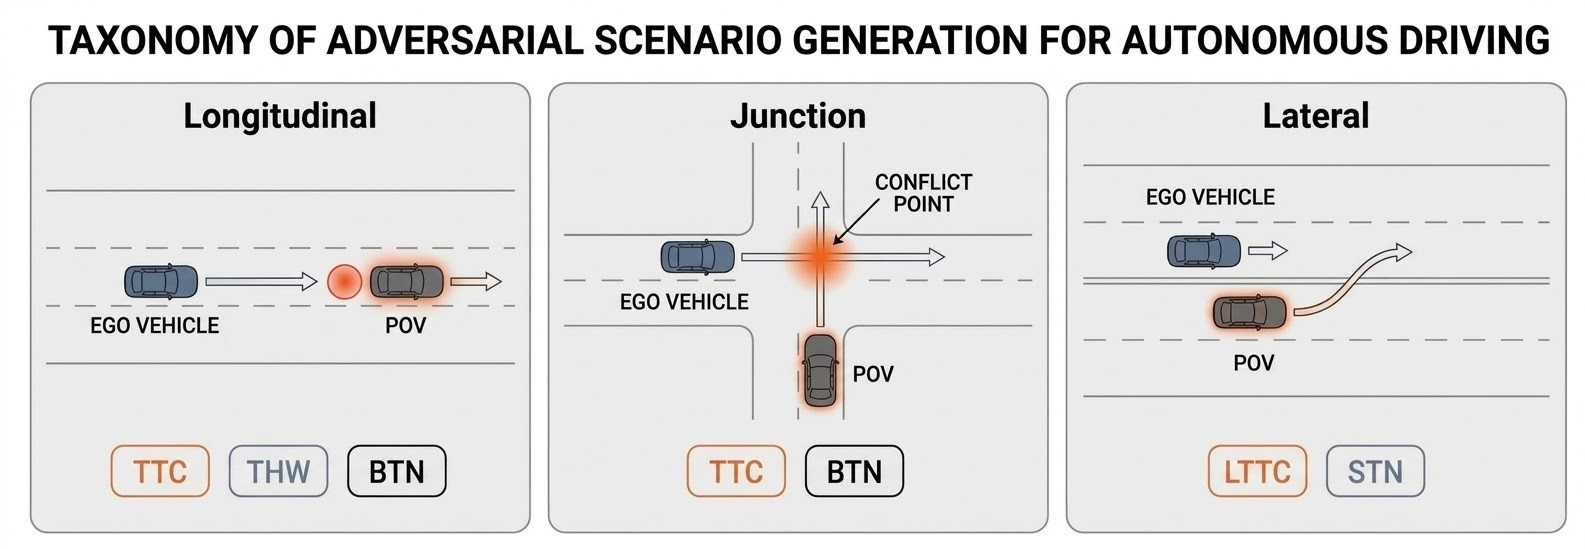
\includegraphics[width=\linewidth]{imgs/scenario_taxonomy.png}
    \caption{Visual taxonomy of the three kinematic categories, their spatial configurations, associated threat metrics, and adversarial generation strategies.}

    \label{fig:scenario_taxonomy}
\end{figure}
\begin{table*}[t]
  \caption{Categorization of NHTSA Pre-Crash Scenarios and Target Threat Metrics}
  \label{tab:kinematic_categories}
  \renewcommand{\arraystretch}{1.0} 
  \begin{tabularx}{\textwidth}{@{} 
      >{\hsize=0.25\hsize\raggedright\arraybackslash}X 
      >{\hsize=0.50\hsize\raggedright\arraybackslash}X 
      >{\hsize=0.25\hsize\raggedright\arraybackslash}X 
      @{}}
    \toprule
    \textbf{Kinematic Category} & \textbf{Included Typologies (NHTSA)} & \textbf{Target Metrics} \\
    \midrule
    
    \rowcolor{blue!5}
    \textbf{Longitudinal} & 
    (1) Lead Vehicle Stopped \newline 
    (2) Lead Vehicle Decelerating \newline 
    (3) Lead Veh. Moving at Lower Speed & 
    TTC, THW, BTN \\
    
    \rowcolor{green!5}
    \textbf{Junction} & 
    (4) Veh. Turning at Non-Signalized \newline 
    (5) Straight Crossing Non-Signalized \newline 
    (6) LTAP/OD at Signalized \newline 
    (7) LTAP/OD at Non-Signalized & 
    TTC, BTN \\
    
    \rowcolor{orange!5}
    \textbf{Lateral} & 
    (8) Veh. Changing Lanes (Same Dir.) \newline 
    (9) Veh. Turning (Same Dir.) \newline
    (10) Vehicle Drifting (Same Dir.) & 
    LTTC, STN \\
    
    \bottomrule
  \end{tabularx}
\end{table*}

% \begin{table*}[t]
%   \caption{Categorization of NHTSA Pre-Crash Scenarios and Target Threat Metrics}
%   \label{tab:kinematic_categories}
%   \renewcommand{\arraystretch}{1.2} 
%   \begin{tabularx}{\textwidth}{@{} 
%       >{\hsize=0.25\hsize\raggedright\arraybackslash}X 
%       >{\hsize=0.50\hsize\raggedright\arraybackslash}X 
%       >{\hsize=0.25\hsize\raggedright\arraybackslash}X 
%       @{}}
%     \toprule
%     \textbf{Kinematic Category} & \textbf{Included Typologies (NHTSA)} & \textbf{Target Metrics} \\
%     \midrule
    
%     \rowcolor{blue!5}
%     \textbf{Longitudinal} & 
%     (1) Lead Vehicle Stopped \newline 
%     (2) Lead Vehicle Decelerating \newline 
%     (3) Lead Veh. Moving at Lower Speed & 
%     TTC, THW, BTN \\
%     \addlinespace
    
%     \rowcolor{green!5}
%     \textbf{Junction} & 
%     (4) Veh. Turning at Non-Signalized \newline 
%     (5) Straight Crossing Non-Signalized \newline 
%     (6) LTAP/OD at Signalized \newline 
%     (7) LTAP/OD at Non-Signalized & 
%     TTC, BTN \\
%     \addlinespace
    
%     \rowcolor{orange!5}
%     \textbf{Lateral} & 
%     (8) Veh. Changing Lanes (Same Dir.) \newline 
%     (9) Veh. Turning (Same Dir.) \newline
%     (10) Vehicle Drifting (Same Dir.) & 
%     LTTC, STN \\
    
%     \bottomrule
%   \end{tabularx}
% \end{table*}
We select ten pre-crash typologies from the NHTSA Pre-Crash Scenario Typology for Crash Avoidance Research~\cite{noauthor_pre-crash_nodate}, drawing from two-vehicle crash scenarios ranked by frequency of occurrence. The nine highest-frequency typologies are retained directly: (1)~Lead Vehicle Stopped (20.46\%), (2)~Vehicle(s) Turning at Non-Signalized Junctions (10.83\%), (3)~Lead Vehicle Decelerating (8.96\%), (4)~Vehicle(s) Changing Lanes -- Same Direction (7.62\%), (5)~Straight Crossing Paths at Non-Signalized Junctions (6.52\%), (7)~Vehicle(s) Turning -- Same Direction (5.68\%), (8)~LTAP/OD at Signalized Junctions (5.29\%), (9)~Lead Vehicle Moving at Lower Constant Speed (4.82\%), and (10)~LTAP/OD at Non-Signalized Junctions (4.68\%). Together, these nine scenarios account for approximately 71\% of all two-vehicle light-vehicle crashes. The sixth-ranked typology, Running Red Light (6.02\%), is excluded because it constitutes an explicit traffic rule violation rather than a legitimate driving behaviour which falls outside this scope, and would be more appropriately addressed through traffic signal compliance testing rather than kinematic perturbation of the POV. In its place, we include the thirteenth-ranked typology, Vehicle(s) Drifting -- Same Direction (2.35\%), which complements the lateral kinematic category by introducing a gradual lane encroachment maneuver distinct from the abrupt lane changes captured by typology~4. This substitution ensures comprehensive coverage of lateral conflict dynamics while maintaining a physically parameterizable search space across all ten selected typologies. The ten typologies are grouped into three kinematic categories --- longitudinal, junction, and lateral --- based on the dominant conflict direction, as summarised in Table~\ref{tab:kinematic_categories} and illustrated in Fig.~\ref{fig:scenario_taxonomy}. Each category is associated with a distinct set of threat metrics that govern the objective function for scenario generation.
\begin{figure*}[t]
    \centering
    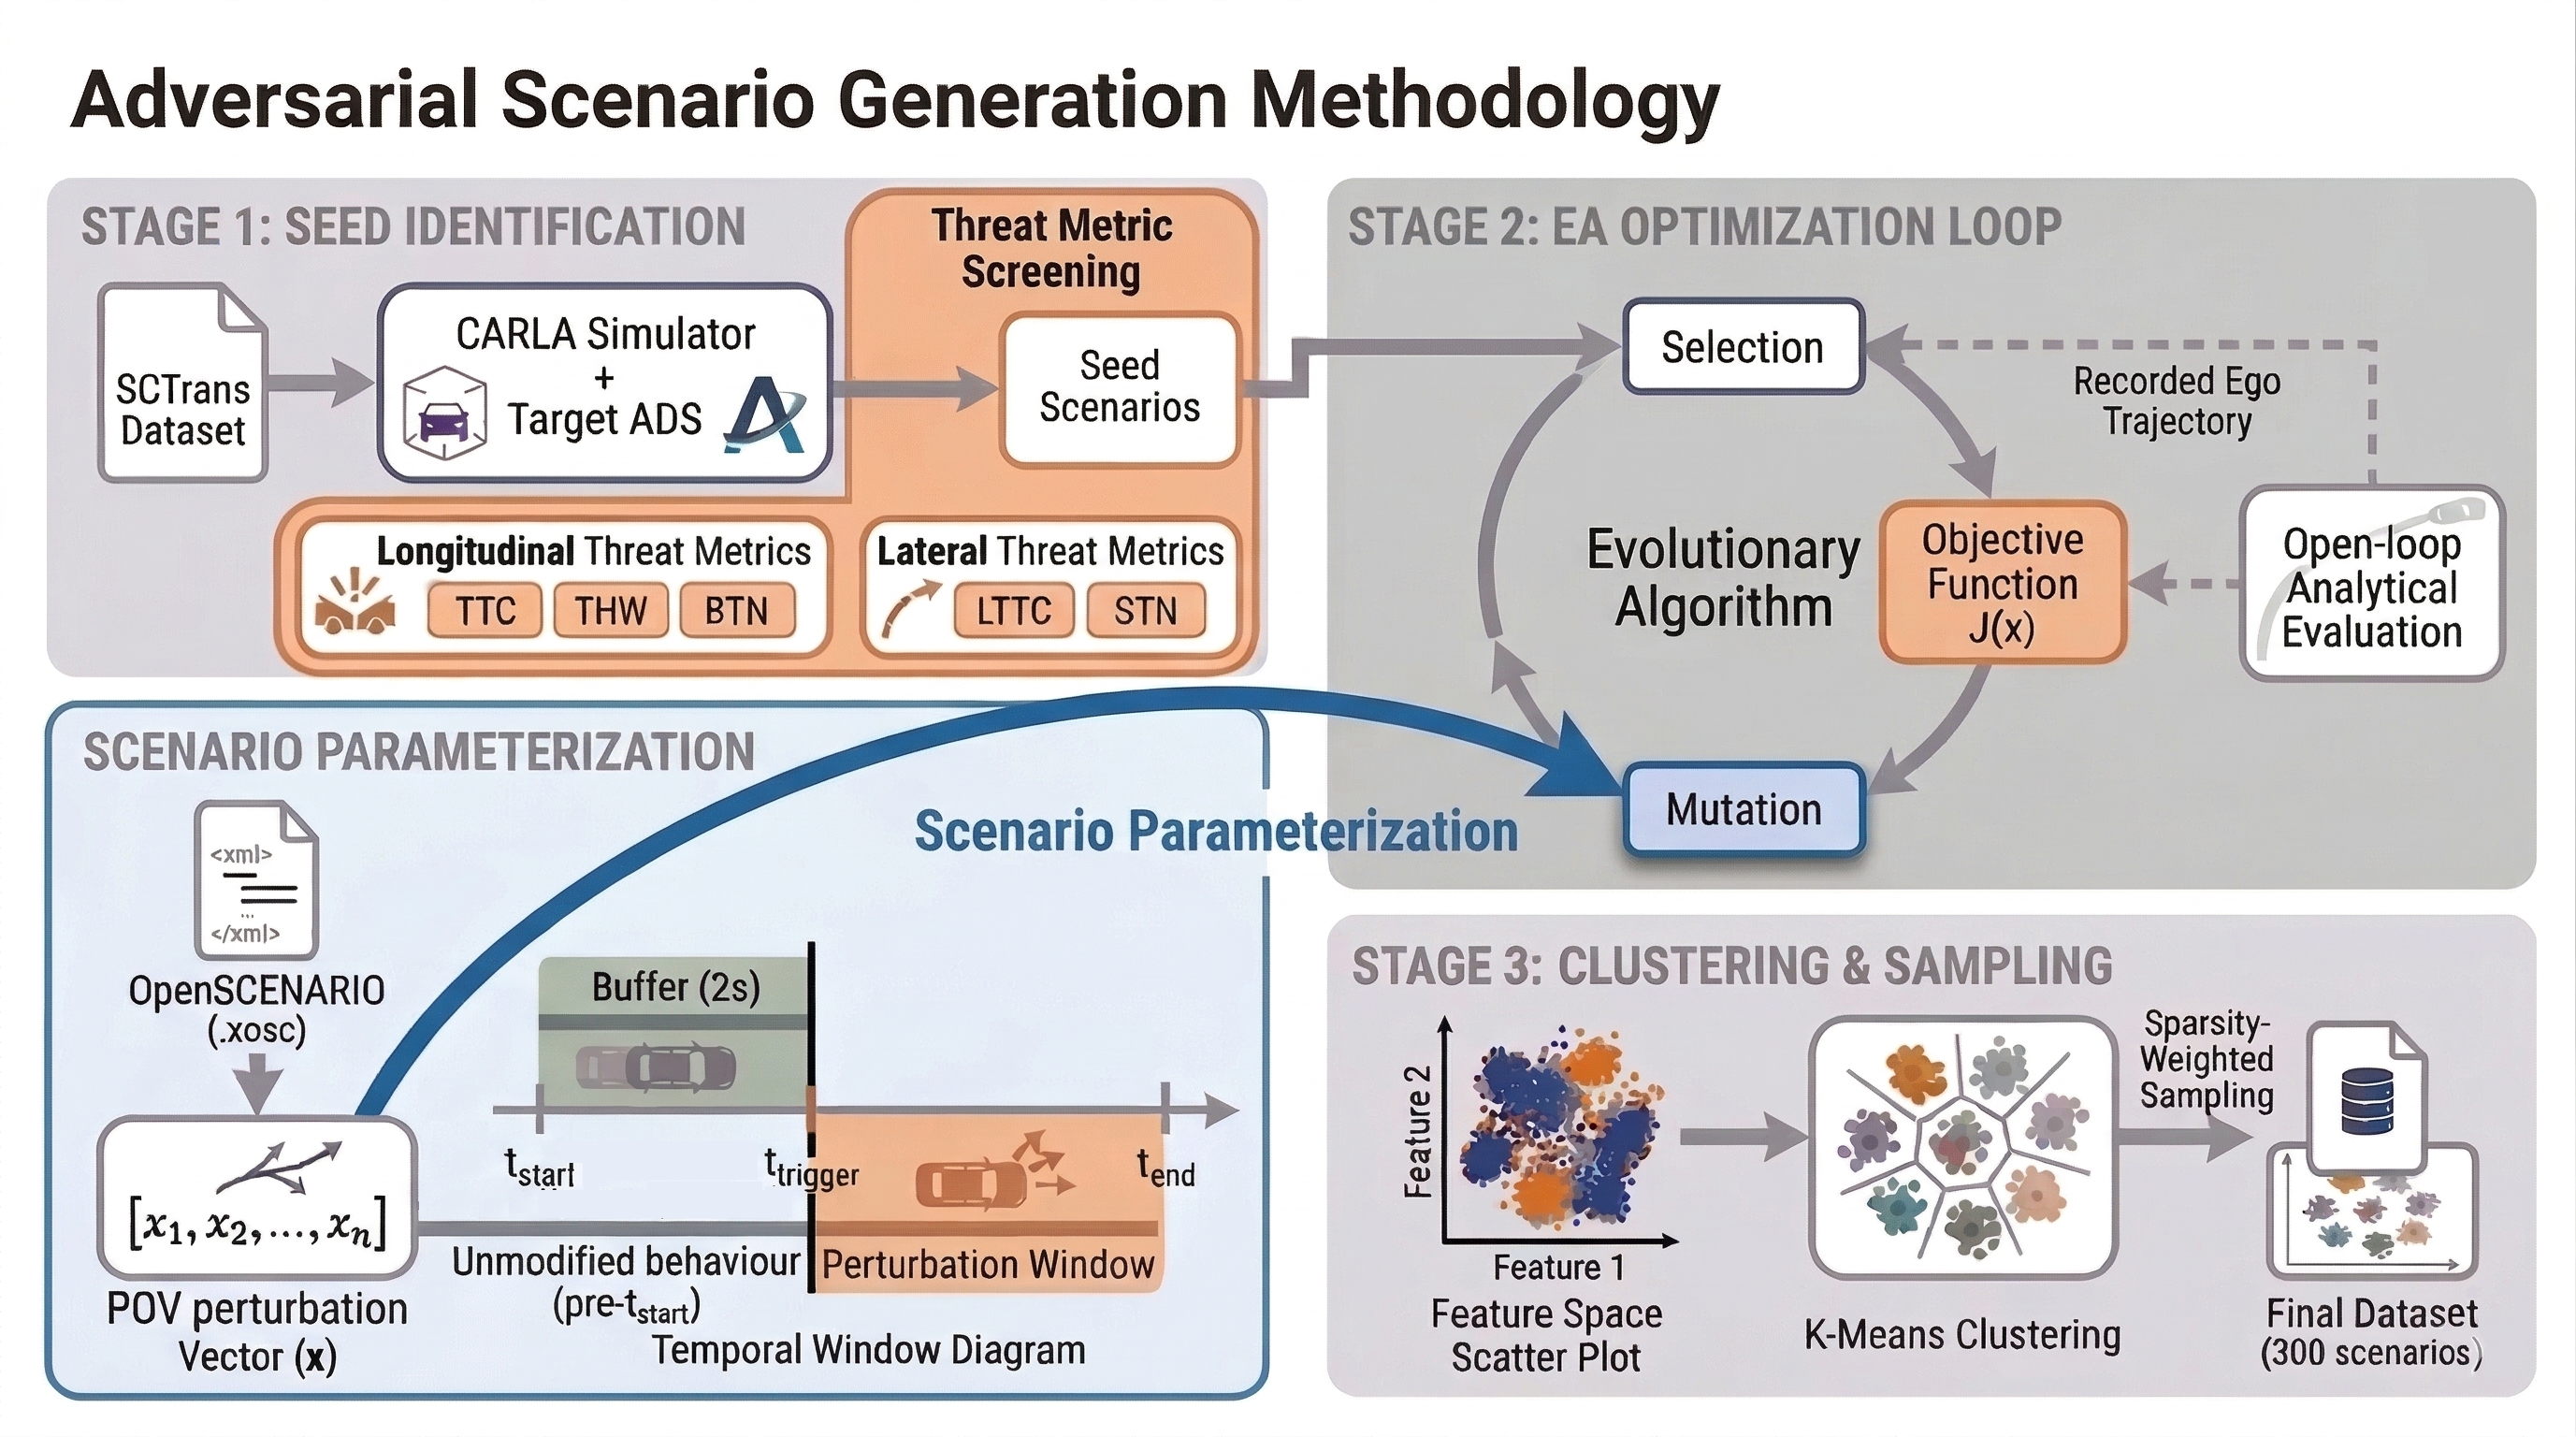
\includegraphics[width=0.8\textwidth]{imgs/generation_workflow.jpg}
    \caption{Overview of the adversarial scenario generation pipeline: seed identification via threat metric screening, scenario parameterization with temporal windowing, evolutionary algorithm optimization using open-loop analytical evaluation, and diversity-driven clustering and sampling.}

    \label{fig:generation_workflow}
\end{figure*}

\subsection{Threat Metrics and Threshold Selection}
\label{sec:threshold_selection}
To identify safety-critical scenarios from the broader dataset, we require a principled method for quantifying collision risk during baseline simulations. We employ five kinematic threat metrics grouped by the dominant conflict direction. The metrics and their associated thresholds provide the quantitative foundation for both seed scenario identification and adversarial scenario evaluation.
\subsubsection{Threat Metric Definitions}
\label{sec:threat_metrics}

For longitudinal and junction conflicts, we define three metrics that capture temporal proximity and braking demand. Time-to-Collision (TTC) and Time Headway (THW) measure the temporal margin available to the ego vehicle, while the Brake Threat Number (BTN) quantifies the required deceleration relative to the vehicle's physical braking limit:
\begin{equation}
    \text{TTC} = \frac{x_{rel}}{v_{x, rel}}, \quad \text{THW} = \frac{x_{rel}}{v_{ego}}, \quad \text{BTN} = \frac{a_{x, req}}{a_{x, max}}
\end{equation}
where $x_{rel}$ and $v_{x, rel}$ are the relative longitudinal distance and velocity, $v_{ego}$ is the ego vehicle's speed, $a_{x, req}$ is the required deceleration to avoid collision, and $a_{x, max}$ is the vehicle's maximum physical braking limit. Lower TTC and THW values indicate greater temporal urgency, while higher BTN values indicate greater braking severity. To prevent mathematical instability when $v_{x, rel}$ approaches zero, the upper bounds of TTC and THW are capped at their corresponding critical thresholds as specified in Table~\ref{tab:thresholds}.

For lateral conflicts such as lane changing and drifting, $v_{x, rel}$ approaches zero, rendering TTC mathematically unstable. We therefore substitute the longitudinal metrics with Lateral Time-to-Collision (LTTC) and Steering Threat Number (STN):
\begin{equation}
    \text{LTTC} = \frac{y_{rel}}{v_{y, rel}}, \quad \text{STN} = \frac{a_{y, req}}{a_{y, max}}
\end{equation}
where $y_{rel}$ and $v_{y, rel}$ are the relative lateral distance and velocity, $a_{y, req}$ is the required lateral evasion acceleration, and $a_{y, max}$ is the maximum lateral acceleration capacity governed by road friction limits. The assignment of metrics to kinematic categories follows Table~\ref{tab:kinematic_categories}.

\subsubsection{Threshold Selection}
\label{sec:thresholds}
Each metric is assigned a two-tier threshold structure. The \textit{critical} tier identifies the onset of a safety-relevant interaction and is used to filter baseline simulations for near-miss events that serve as seed scenarios for adversarial generation. The \textit{emergency} tier defines the boundary of an unavoidable conflict and serves as the threat threshold for the optimisation process: candidate scenarios must drive at least one metric beyond its emergency threshold to be retained. The threshold values, summarised in Table~\ref{tab:thresholds}, are derived from the Euro~NCAP Assisted Driving Highway \& Interurban Test and Assessment Protocol v2.2~\cite{noauthor_euro_nodate}.

\begin{table}[htbp]
\centering
\caption{Threat metric thresholds derived from the Euro~NCAP Assisted Driving Highway \& Interurban Test and Assessment Protocol v2.2~\cite{noauthor_euro_nodate}.}
\label{tab:thresholds}
\renewcommand{\arraystretch}{1.0}
\begin{tabular}{@{}llcl@{}}
\toprule
\textbf{Metric} & \textbf{Level} & \textbf{Value} & \textbf{Derivation Basis} \\
\midrule
\multirow{2}{*}{TTC}
  & Critical  & 3.0  & ACC abort criterion (\S3.3.1.1)          \\
  & Emergency & 1.5  & FCW issuance threshold (\S4.3.1)         \\
\multirow{2}{*}{THW}
  & Critical  & 2.0  & ISO~15622 upper bound   \\
  & Emergency & 1.0  & ACC minimum gap (\S3.3.1.1)   \\
\multirow{2}{*}{BTN}
  & Critical  & 0.52 & CCRs (\S3.3.1) \\
  & Emergency & 0.80 & ACC-to-AEB transition (\S4.3.1)   \\
\multirow{2}{*}{LTTC}
  & Critical  & 1.5  & Cut-in TTC (\S3.3.1.3)   \\
  & Emergency & 0.5  & C2MC cut-in TTC (\S3.3.2.5) \\
\multirow{2}{*}{STN}
  & Critical  & 0.40 & Lane Support System (\S4.3.5) \\
  & Emergency & 0.64 & S-Bend (\S3.4.1) \\
\bottomrule
\end{tabular}
\end{table}

% \begin{table}[htbp]
% \centering
% \caption{Threat metric thresholds for autonomous driving scenario evaluation, derived from the Euro~NCAP Assisted Driving Highway \& Interurban Test and Assessment Protocol v2.2~\cite{noauthor_euro_nodate}.}
% \label{tab:thresholds}
% \renewcommand{\arraystretch}{1.3}
% \begin{tabular}{@{}llcl@{}}
% \toprule
% \textbf{Metric} & \textbf{Level} & \textbf{Value} & \textbf{Derivation Basis} \\
% \midrule
% \multirow{2}{*}{TTC}
%   & Critical  & 3.0  & ACC abort criterion (\S3.3.1.1)          \\
%   & Emergency & 1.5  & FCW issuance threshold (\S4.3.1)         \\
% \midrule
% \multirow{2}{*}{THW}
%   & Critical  & 2.0  & ISO~15622 upper bound   \\
%   & Emergency & 1.0  & ACC minimum gap (\S3.3.1.1)   \\
% \midrule
% \multirow{2}{*}{BTN}
%   & Critical  & 0.52 & CCRs (\S3.3.1) \\
%   & Emergency & 0.80 & ACC-to-AEB transition (\S4.3.1)   \\
% \midrule
% \multirow{2}{*}{LTTC}
%   & Critical  & 1.5  & Cut-in TTC (\S3.3.1.3)   \\
%   & Emergency & 0.5  & C2MC cut-in TTC (\S3.3.2.5) \\
% \midrule
% \multirow{2}{*}{STN}
%   & Critical  & 0.40 & Lane Support System (\S4.3.5) \\
%   & Emergency & 0.64 & S-Bend (\S3.4.1) \\
% \bottomrule
% \end{tabular}
% \end{table}

Of the ten threshold values, four (TTC critical and emergency, LTTC critical and emergency) are directly mapped from explicitly stated protocol parameters --- test abort criteria, warning issuance deadlines, and prescribed TTC values at lane-change completion. The remaining six are derived from the protocol's test configurations through established physical relationships: THW values from the closest following distance requirement, BTN values from the most demanding ACC scenario (CCRs) and the ACC-to-AEB transition boundary, and STN values from the LKA departure threshold and the S-Bend lateral acceleration demand.
% \subsubsection{Threshold Selection}
% \label{sec:thresholds}

% Each metric is assigned a two-tier threshold structure. The \textit{critical} tier identifies the onset of a safety-relevant interaction and is used to filter baseline simulations for near-miss events that serve as seed scenarios for adversarial generation. The \textit{emergency} tier defines the boundary of an unavoidable conflict and serves as the threat threshold for the optimisation process: candidate scenarios must drive at least one metric beyond its emergency threshold to be retained. The threshold values, summarised in Table~\ref{tab:thresholds}, are derived from the Euro~NCAP Assisted Driving Highway \& Interurban Test and Assessment Protocol v2.2~\cite{noauthor_euro_nodate}.

% \begin{table}[htbp]
% \centering
% \caption{Threat metric thresholds for autonomous driving scenario evaluation, derived from the Euro~NCAP Assisted Driving Highway \& Interurban Test and Assessment Protocol v2.2~\cite{noauthor_euro_nodate}.}
% \label{tab:thresholds}
% \renewcommand{\arraystretch}{1.3}
% \begin{tabular}{@{}llcl@{}}
% \toprule
% \textbf{Metric} & \textbf{Level} & \textbf{Value} & \textbf{Derivation Basis} \\
% \midrule
% \multirow{2}{*}{TTC}
%   & Critical  & 3.0  & ACC abort criterion (\S3.3.1.1)          \\
%   & Emergency & 1.5  & FCW issuance threshold (\S4.3.1)         \\
% \midrule
% \multirow{2}{*}{THW}
%   & Critical  & 2.0  & ISO~15622 upper bound   \\
%   & Emergency & 1.0  & ACC minimum gap (\S3.3.1.1)   \\
% \midrule
% \multirow{2}{*}{BTN}
%   & Critical  & 0.52 & CCRs (\S3.3.1) \\
%   & Emergency & 0.80 & ACC-to-AEB transition (\S4.3.1)   \\
% \midrule
% \multirow{2}{*}{LTTC}
%   & Critical  & 1.5  & Cut-in TTC (\S3.3.1.3)   \\
%   & Emergency & 0.5  & C2MC cut-in TTC (\S3.3.2.5) \\
% \midrule
% \multirow{2}{*}{STN}
%   & Critical  & 0.40 & Lane Support System (\S4.3.5) \\
%   & Emergency & 0.64 & S-Bend (\S3.4.1) \\
% \bottomrule
% \end{tabular}
% \end{table}

% Of the ten threshold values, four are \textit{directly mapped} from explicitly stated protocol parameters. The TTC critical threshold of 3.0\,s corresponds to the test abort criterion specified in (\S3.3.1.1), whereby a trial is terminated if the ACC system has not initiated braking by this point. The TTC emergency threshold of 1.5\,s is the forward collision warning (FCW) issuance deadline in (\S4.3.1), below which partial credit is awarded only if a warning has been provided. The LTTC thresholds of 1.5\,s and 0.5\,s correspond directly to the prescribed TTC values at lane-change completion for the car-to-car cut-in test (\S3.3.1.3) and the car-to-motorcyclist cut-in test (\S3.3.2.5), respectively.

% The remaining six thresholds are \textit{derived} from the protocol's test configurations through established physical relationships. The THW values of 2.0\,s (critical) and 1.0\,s (emergency) are inferred from the protocol's requirement to test at the ``closest following distance'' (\S3.3.1.1). The BTN critical value of 0.52 is computed from the most demanding ACC scenario---CCRs. The BTN emergency value of 0.80 marks the transition into the AEB operating regime, where deceleration demands exceed the ACC comfort boundary. The STN critical value of 0.40 is mapped from the protocol's LKA departure threshold (\S4.3.5), which awards points only when lane departure is limited to 0.4\,m. The STN emergency value of 0.64 is derived from the lateral acceleration demand of the S-Bend second turn.

\subsection{Adversarial Scenario Generation -- Regular Setting}\label{sec:generation}
Building on the ten target typologies and their associated threat metrics defined in Sec.~\ref{sec:typology_selection} and~\ref{sec:threshold_selection}, this section presents the adversarial scenario generation pipeline. The core objective is to transform near-miss traffic events into more critical, collision-likely test cases without violating physical plausibility. An overview of the complete pipeline is illustrated in Fig.~\ref{fig:generation_workflow}. The pipeline begins with an empirical screening phase, simulating 854 real-world traffic events from the SCTrans dataset in the CARLA simulator to identify vulnerable ``seed'' scenarios which trigger the predefined threat metrics corresponding to each typology. We frame the adversarial generation as a constrained optimization problem. By parameterizing the dynamic behavior of the Principal Other Vehicle (POV) within the OpenSCENARIO framework and constraining these bounds to Euro NCAP regulatory standards, we maintain strict kinematic realism. An evolutionary algorithm (EA) iteratively perturbs these variables using open-loop analytical evaluation against recorded ego-vehicle trajectories, guided by the typology-specific objective function. A key contribution of this methodology is the open-loop analytical optimization with temporally scoped perturbations (Sec.~\ref{sec:seed}): by restricting modifications to the threat-metric-triggered window and evaluating against recorded baseline trajectories, we achieve efficient search-space exploration while maintaining the physical validity of each generated scenario. Finally, feature-space clustering with sparsity-weighted sampling distills the results into 300 highly diverse, representative failure modes across all ten typologies.

\subsubsection{Seed Scenario Identification and Parameterization}\label{sec:seed}
% \subsection{Adversarial Behaviours Supported}
% - include a table on the different types of adversarial behaviour


The adversarial generation pipeline begins with the empirical identification of high-risk baseline events. We execute 854 original, unperturbed scenarios from the SCTrans dataset within the CARLA simulator, utilizing Apollo as the target ego vehicle. During these baseline simulations, we continuously monitor the kinematic interactions between the ego vehicle and the surrounding traffic. Scenarios that breach safe operational thresholds and trigger our target threat metrics (TTC, THW, and BTN for longitudinal conflicts; LTTC and STN for lateral conflicts) are classified as near-misses and extracted as foundational ``seed'' scenarios. The threshold values defining these near-miss boundaries are established in Sec~\ref{sec:threshold_selection}.

Once these vulnerable seeds are identified, their existing OpenSCENARIO (\texttt{.xosc}) definitions are restructured to decouple the static environment from the parameterized adversarial agent. The map topology, defined in the corresponding \texttt{.xodr} files, remains unchanged. Static environmental constraints and background non-POV traffic within the \texttt{.xosc} files are preserved, constrained to their recorded trajectories, to maintain the baseline realism of the SCTrans data. Conversely, the dynamic state of the Principal Other Vehicle (POV)---the primary adversarial agent---is parameterized to form a continuous search space. Crucially, we do not modify the entire scenario timeline. For each seed, we identify the temporal window during which the threat metrics are actively triggered, and restrict perturbations exclusively to this window plus a 2-second preceding buffer. This buffer allows the POV to transition smoothly from its unmodified baseline behavior to the perturbed, higher-risk state. All behavior prior to this window remains identical to the original scenario, ensuring that the ego vehicle's recorded trajectory up to the onset of the perturbation window is valid and unaffected.

We define a perturbation vector $\mathbf{x}$ for each seed, encompassing variables such as the POV's initial velocity ($v_{POV}$) and acceleration profiles ($a_{POV}$). We utilize OpenSCENARIO triggers, specifically the \texttt{RelativeDistanceCondition}, \texttt{RelativeSpeedCondition}, to define the exact spatial and velocity thresholds at which the POV executes risky behaviors, such as a sudden brake within a critical time window when the ego vehicle is trailing, or an aggressive lane change. By directly modifying these parameters within the \texttt{.xosc} XML structure, we create a controllable testbed ready for heuristic optimization.

\subsubsection{Defining the Objective Function}\label{sec:objective}
To guide the search algorithm toward a collision state, we formulate a fitness function $J(\mathbf{x})$ that quantitatively evaluates the danger of each candidate trajectory. The function is designed such that lower values of $J(\mathbf{x})$ indicate higher collision risk, and the evolutionary algorithm seeks to minimize it. The unified objective function is formulated as:
\begin{equation}
    J(\mathbf{x}) = \sum_{i} \mathcal{T}_{i}(\mathbf{x}) - \sum_{j} \mathcal{R}_{j}(\mathbf{x})
\end{equation}
where $\mathcal{T}_{i}(\mathbf{x})$ denotes the time-based proximity metrics (TTC/THW for longitudinal conflicts, or LTTC for lateral conflicts) and $\mathcal{R}_{j}(\mathbf{x})$ denotes the threat number metrics (BTN for longitudinal conflicts, or STN for lateral conflicts), as defined in Sec.~\ref{sec:threat_metrics}. The time-based metrics decrease as collision risk increases, while the threat numbers increase with risk; subtracting the latter ensures that all terms contribute consistently toward a lower $J(\mathbf{x})$ for higher-risk scenarios. All metrics are weighted equally, as they capture complementary aspects of collision risk: temporal margins and the required evasive effort. Minimizing $J(\mathbf{x})$ therefore simultaneously drives the scenario toward shorter time margins and greater difficulty for the ego vehicle to avoid collision.

\subsubsection{Optimization and Search Algorithm}\label{sec:optimization}
We model the generation pipeline as a constrained optimization problem, utilizing an Evolutionary Algorithm (EA) to iteratively evolve the perturbation vector $\mathbf{x}$ toward a critical collision boundary. To ensure that perturbed trajectories remain physically plausible, the allowable boundaries for $\mathbf{x}$ are strictly constrained according to the Euro NCAP AD Test and Assessment Protocol v2.2, ensuring that every generated scenario represents a standardized, kinematically valid testing condition rather than an edge-case simulator artifact. This optimization phase operates entirely through open-loop analytical evaluation rather than closed-loop simulation, enabling efficient and broad search-space exploration.

We use the ego-vehicle trajectory recorded during the preliminary baseline simulation in CARLA. For every candidate generated by the EA, we analytically superimpose the perturbed POV behavior onto this recorded trajectory. As described in Sec.~\ref{sec:seed}, perturbations are restricted to the threat-metric-triggered window and its preceding 2-second buffer, ensuring that the ego vehicle's behavior prior to this window remains identical to the baseline. By evaluating the ego vehicle in this open-loop manner---without factoring in closed-loop evasive responses---the EA is directed toward scenarios that are analytically more critical than the original seeds.

The EA employs a standard evolutionary loop: parent selection is performed across the full candidate pool, and mutation is applied to a sampled 10\% of the population at each generation to introduce controlled variation while preserving the majority of high-fitness solutions. The fitness function $J(\mathbf{x})$ evaluates the analytically superimposed trajectories using the typology-specific threat metrics to quantify the collision risk. The EA selects the parameter combinations yielding the lowest $J(\mathbf{x})$ to breed the next generation, continuously refining the POV's adversarial behavior. The EA terminates once it has collected a sufficient pool of 100 candidate scenarios that surpass at least one threat threshold for each typology. This threshold serves as a quality floor, ensuring all retained scenarios represent a meaningful increase in risk over their original seeds, while preserving diversity in the solution space for the subsequent clustering stage. The specific threat threshold values are detailed in Sec.~\ref{sec:threshold_selection} and Sec.~\ref{sec:objective}.

\subsubsection{Clustering and Selection}
Once the evolutionary algorithm produces a large pool of high-risk candidates, we distill these results into a highly diverse, non-redundant dataset. For each of the ten NHTSA typologies, the EA generates a pool of 100 candidate scenarios, each surpassing the predefined threat threshold. We then extract the kinematic features of each scenario at the point of highest threat, such as the relative speed, approach angle, and required ego-vehicle deceleration. Unlike the threat metrics used in the fitness function, which quantify pre-crash risk during optimization, these features characterize the physical crash outcome and are therefore better suited for distinguishing between structurally different failure modes. For each typology, these features are mapped into a multi-dimensional feature space and grouped using a K-Means clustering algorithm based on physical and kinetic similarity. To select the 30 representative scenarios per typology, we employ sparsity-weighted sampling: the algorithm probabilistically favors scenarios with greater distance to their nearest neighbor in feature space. This per-typology process yields a final dataset of 300 scenarios (30 $\times$ 10 typologies) that captures a wide spectrum of failure modes while avoiding redundant crash dynamics.


\subsection{Adversarial Scenario Generation for Roundabout Maps}
Roundabouts represent a particularly demanding class of road geometry for autonomous systems, owing to their continuous merging dynamics, curved lane structures, and the absence of conventional traffic signals. Existing scenario datasets such as ScTrans do not contain roundabout environments, necessitating a bespoke pipeline for roundabout adversarial scenario generation. This pipeline proceeds in four stages: map acquisition and validation, roundabout geometry identification, baseline scenario generation, and adversarial behaviour injection.

\subsubsection{Roundabout Map Generation}
To obtain a diverse set of real-world roundabout layouts, the OpenStreetMap Overpass API was used to retrieve map data for roundabouts located in France — selected for its right-hand drive network and high roundabout density. Retrieved maps were converted from OSM format to the OpenDRIVE (XODR) standard using SUMO's \texttt{netconvert} tool and filtered to retain only the geometry relevant to each roundabout and its immediate approaches. Each candidate map was then automatically validated within CARLA by spawning vehicles across all road segments to identify geometry errors such as malformed or disconnected lanes. Maps passing automated validation were further subject to manual inspection via bird's-eye screenshots before inclusion in the scenario pool. A total of 12 maps were selected for scenario generation.

\subsubsection{Roundabout Geometry Identification}
Identifying the functional geometry of a roundabout, namely its entrances, exits, and lane structure, is essential for scenario generation and adversary logic. We exploit CARLA's waypoint-based road network interface, which allows the road network to be treated as a set of directed graphs amenable to standard search algorithms. Entrances and exits are identified via forward and reverse traversal respectively: at each branch point, a lookahead with a larger step distance classifies paths deviating from the roundabout centre as exits. Adjacent lanes are identified by probing perpendicularly for waypoints sharing the same heading. Suitable vehicle spawn points approaching each entrance are then located to ensure that spawned traffic enters the roundabout naturally. Geometry metadata — roundabout shape, radius, number of entrances and exits, lane counts, and road type — is stored and used to inform subsequent scenario generation.

\subsubsection{Baseline Scenario Generation}

Validated maps serve as the basis for baseline scenarios representing normal, safe driving behaviour. Each scenario assigns the ego vehicle and background traffic random spawn points and destinations from the pre-computed spawn point set, with the ego vehicle's spawn constrained to lie outside the roundabout to ensure that each run covers both entry and exit. No traffic is filtered and no phase is fast-forwarded, reflecting the compounding interdependencies characteristic of roundabout environments.

Prior to inclusion, each candidate scenario is assessed for \textit{interestingness} that checks whether adversarial behaviours have a meaningful opportunity to activate and influence the ego vehicle. This is evaluated over two simulation passes: a baseline pass with no adversaries, and a probing pass in which adversary vehicles report the internal metrics by which triggered behaviours would activate. A scenario is classified as interesting if (1) the ego vehicle's behaviour differs between the two passes, and (2) triggered behaviours had an opportunity to activate. Where a triggered behaviour approached but did not reach its activation threshold, the adversary's spawn point is adjusted along the road based on the gradient between the activation metric and proximity to the ego vehicle, and the simulation is re-run. Scenarios for which no viable adjustment exists are discarded and regenerated.

\subsubsection{Adversarial Behaviours}
Point-to-point navigation is handled by CARLA's Traffic Manager, above which a meta-controller layer is implemented to govern lane selection, exit manoeuvres, and dynamic adjustments to speed, acceleration, and following distance on roundabouts. All adversarial behaviour is implemented at this layer. Adversarial behaviours are divided into two categories: \textit{constant behaviours}, which apply persistent modifications to a vehicle's driving parameters (e.g. increased speed, reduced following distance), and \textit{triggered behaviours}, which initiate a specific dangerous event in response to a defined condition. To approximate realistic traffic variability, each adversary is assigned a speed and acceleration profile drawn from a narrow distribution around the target parameters. The supported typologies are as follows.
\begin{description}
\item[Lead Vehicle Stopped (Triggered)] The adversary performs an emergency braking manoeuvre while directly ahead of the ego vehicle, triggered upon detecting ego vehicle proximity within a defined threshold.
\item[Lead Vehicle Decelerating (Triggered)] Similar to Lead Vehicle Stopped, but the adversary decelerates to a fraction of its current speed rather than coming to a complete halt.
\item[Vehicle(s) Changing Lanes(Triggered)] The adversary enters the roundabout in a lane inappropriate for its intended exit, then performs an unsignalled lane change into the ego vehicle's path when passing alongside it.
\item[Lead Vehicle at Lower Constant Speed (Constant)] The adversary's target speed is set below the posted speed limit, causing it to travel consistently slower than baseline traffic.
\item[Control Loss(Triggered)] When the adversary's trajectory is predicted to intersect with the ego vehicle, all control inputs are ceased, modelling a loss-of-control event.
\item[Speeding (Constant)] The adversary's target speed is set above the posted speed limit.
\item[Tailgating (Constant)] The adversary maintains an unsafe following distance, reducing headway below the safe threshold.
\end{description}

\subsubsection{Threat Metrics}

The three threat metrics — Time Headway (THW), Time to Collision (TTC), and Brake Threat Number (BTN) — employ the same fundamental calculations as described in Sec.~\ref{sec:threshold_selection}, adapted for the curved trajectories typical of roundabout driving. Longitudinal headway is computed along the ego vehicle's lane path, and collision predictions are derived from the intersection of vehicle trajectories modelled as quadratics, with vehicles represented by their full bounding boxes rather than point approximations.

In total, thirty scenarios are generated per adversarial typology across nine behaviour categories, with ten simulation repetitions per configuration, yielding 2,700 simulation runs completed in approximately 30 hours of simulator time.
\iffalse
\subsection{Adversarial Scenario Generation for Roundabout Maps}
We use a tailored approach for generating adversarial scenarios targeting roundabouts. This is because existing scenario datasets like ScTrans, do not contain any roundabouts. Roundabouts represent a particularly demanding class of road geometry for autonomous systems, owing to their continuous merging dynamics, curved lane structures, and the absence of conventional traffic signals. For the rounabout setting, we have to first generate roundabout maps, identify their geometry and then design baseline scenarios with these maps. We then go on to modify these baseline scenarios to introduce adversarial POV behaviours from Table~\ref{}.   

\subsubsection{Roundabout Map Generation.}
Roundabout scenarios require high fidelity map geometry that can be loaded into the driving simulator. To obtain a diverse set of real-world roundabout layouts, the OpenStreetMap Overpass API was used to obtain data for roundabouts located in France, selected due to its right hand drive road network and high density of roundabouts, for a large and varied sample of geometries. The retrieved map data, in OSM format, was converted to the OpenDRIVE (XODR) standard using SUMO's netconvert tool and subsequently filtered to retain only the geometry relevant to each roundabout and its immediate approaches.

Each candidate roundabout map was then automatically validated within the CARLA simulator. The centre of each roundabout was converted to CARLA's co-ordinate system and the roundabout geometry was identified as described in the next paragraph. Vehicles were spawned and directed to drive across all road segments of the map in order to identify geometry errors, such as malformed road segments or disconnected lanes. Finally, a bird's-eye screenshot of each validated map was generated for manual inspection and inclusion in the scenario pool.

\subsubsection{Roundabout Geometry Identification.}
Identifying the functional geometry of a roundabout- its entrances, exits, and lane structure- is essential for scenario generation and adversary logic. CARLA provides a waypoint-based interface to the road network: any point on the drivable surface can be resolved to a waypoint, and each waypoint supports forward and backward traversal at a specified step distance, returning all reachable successors or predecessors where the network branches. This effectively allows the road network to be considered as a set of directed graphs, which can be searched by common search algorithms.

Adjacent lanes are identified by probing perpendicularly for waypoints sharing the same heading. Continuous forward traversal with a small step distance from any point on the roundabout identifies all exits and circles around the roundabout to close the loop: at each branch, a lookahead with a much larger step distance is performed and the path(s) that deviates from the roundabout centre is classified as an exit. The same algorithm in reverse identifies all entrances. A further search from each entrance locates suitable spawn points for vehicles approaching the roundabout, ensuring that spawned traffic enter the roundabout naturally.


After geometry identification, the results for roundabout shape, radius, number of entrances, exits, and their lanes, roadtype, and test results were stored and used to select a comprehensive set of maps for scenario generation. We selected 12 maps for scenario generation at the end of this step. 

\subsubsection{Baseline Scenario Generation}

Once a validated roundabout map has been produced, it serves as the basis for generation of baseline scenarios that represent normal, safe driving behaviour. Each scenario is initialised by assigning all vehicles- both the ego vehicle and background traffic- a random spawn point from the pre-calculated spawn points and a random destination offset from an exit to the roundabout. The ego vehicle's spawn point is constrained to lie outside the roundabout itself, ensuring that each successful scenario run covers both entry to and exit from the roundabout.

Scenarios are designed to be as natural and minimally contrived as possible. To this end, no traffic is filtered from the simulation, the simulation is not fast-forwarded past any phase, and all vehicles are spawned at the start of each run. This design choice reflects the fact that, in roundabout environments, the actions of any vehicle can produce compounding effects that are difficult to predict outside of full simulation- for example, a vehicle that never approaches the ego vehicle directly may nevertheless delay another vehicle that subsequently interacts with it.

Before a generated scenario is included in subsequent steps, it is first evaluated for interestingness. An interesting scenario is one in which the ego vehicle meaningfully interacts with other traffic and triggered adversarial behaviours have an opportunity to activate within the run. This assessment is performed in two simulation passes. In the first pass, the ego vehicle drives through the scenario with no adversaries present, establishing a behavioural baseline. In the second pass, adversary vehicles are assigned a special probing behaviour that is functionally identical to the baseline but additionally reports the internal metrics by which triggered behaviours would activate.

For a scenario to be classified as interesting, two conditions must be satisfied: (1) the ego vehicle's driving behaviour must differ between the two passes, indicating that the presence of adversaries influenced its actions; and (2) triggered behaviours must have had an opportunity to activate during the second pass. If the second pass reveals that a triggered behaviour came close to its activation threshold without activating, the corresponding adversary's spawn point is adjusted either forwards or backwards along the road based on the gradient between the activation metric and the adversary's proximity to the ego vehicle, and the simulation is re-run. If no such adjustment is viable, the scenario is discarded and regenerated.


\subsubsection{Roundabout Adversary Behaviours.}
Point-to-point vehicle navigation is handled by CARLA's built-in Traffic Manager module. However, an additional meta-controller layer is implemented above the Traffic Manager to enable more complex and realistic driving behaviour on roundabouts. The meta-controller governs lane selection on entry and during circulation, exit manoeuvres from inner lanes, and dynamic adjustments to each vehicle's maximum speed, acceleration, and following distance. All adversarial behaviour is also implemented on this layer, although often connecting to a central monitor to avoid repeat computations.

Adversarial behaviours are generated by performing small modifications to the baseline interesting scenarios, altering the parameters necessary to produce the desired adversarial typology.
Adversarial behaviours are divided into two categories -- 1. Constant behaviours represent persistent modifications to a vehicle's driving parameters relative to the baseline, such as increased speed or a reduced following distance, 2. Triggered behaviours cause the adversary to initiate a specific dangerous event in response to a defined condition, such as performing an emergency stop or executing an unsafe lane change in the path of another vehicle.
To better approximate realistic traffic conditions, all adversary behaviours incorporate a degree of variation. Each adversary vehicle is assigned a slightly different speed and acceleration profile, drawn from a narrow distribution around the set parameters. 
We describe the different adversarial typologies supported for roundabouts below. 


\paragraph{Lead Vehicle Stopped. (Triggered)}
The adversary performs an emergency braking manoeuvre while directly ahead of the ego vehicle on the roundabout. This behaviour is triggered when the adversary detects that it is being followed by the ego vehicle within a defined proximity threshold.

\paragraph{Lead Vehicle Decelerating. (Triggered)}
This behaviour is similar to Lead Vehicle Stopped, but rather than coming to a complete halt, the adversary decelerates to a fraction of its current speed.

\paragraph{Vehicle(s) Changing Lanes – Same Direction. (Triggered)}
The adversary enters the roundabout in a lane that is inappropriate for its intended exit. When it passes alongside the ego vehicle occupying the correct lane, it performs a lane change without yielding, cutting in front of the ego vehicle.

\paragraph{Lead Vehicle at Lower Constant Speed. (Constant)}
The adversary's target speed is set below the posted speed limit, causing it to travel at a consistently lower speed than a baseline vehicle in the same scenario.

\paragraph{Control Loss Without Prior Vehicle Action. (Triggered)}
When the adversary's trajectory is predicted to result in a collision with the ego vehicle, it ceases all control inputs to the simulation, modelling a situation in which the driver has lost control of the vehicle.

\paragraph{Speeding. (Constant)}
The adversary's target speed is set above the posted speed limit, causing it to travel faster than surrounding traffic.

\paragraph{Tailgating. (Constant)}
The adversary is configured with an unsafe following distance to leading vehicles, reducing its headway below the safe threshold.


\subsubsection{Threat Metrics.}

The three threat metrics considered- Time Headway (THW), Time to Collision (TTC), and Brake Threat Number (BTN)- employ the same fundamental calculations as described in the preceding sections, but are adapted to account for the curved vehicle trajectories typical of roundabout driving. Headway is computed by measuring the distance between vehicles along the path of the ego vehicle's lane, effectively straightening the road segments for the purpose of longitudinal distance measurement. Collision predictions are derived from the intersection of vehicle trajectories modelled as quadratics, with both vehicles represented by their full bounding boxes rather than point approximations.


 In our experiments, we generate thirty roundabout scenarios for each of the nine adversary behaviours, with ten repetitions per configuration, yielding a total of 2,700 simulation runs in approximately 30 hours of simulator time.
\fi
 \iffalse
%Of 26 maps generated, 12 were selected.
%This algorithm fails in the rare case a roundabout has another road intersecting it, typically a bus lane that goes straight through the centre of the roundabout. This can be easily identified and flagged. Such roundabouts need a start point for the search set manually to avoid searching along the road intersecting the roundabout instead of the roundabout itself.
 
\subsubsection{Run Outcome Classification.}

Each simulation run is classified into one of several outcome categories. The two main outcomes are arrived, in which the ego vehicle successfully reaches its destination, and collision, in which the ego vehicle and an adversary physically contacted. An additional outcome is falling off the map, which occurs the ego vehicle leaves the drivable surface- the simulator only treats the road as solid.  A further outcome, halting, is also considered: this occurs when an incident- such as another vehicle blocking the road ahead- prevents the ego vehicle from proceeding until the obstruction is resolved. Halting is not a negative outcome, as it indicates that the ego vehicle responded safely by coming to a controlled stop without causing further collisions, and will continue when it is safe to do so.

It should also be noted that, in contrast to typical junction and straight road scenarios, the minor violation of crossing lane boundaries is much less relevant on roundabouts, as lane transitions are an expected part of normal entry and exit behaviour and roundabout lanes are marked as such.
\fi

% \section{Experiment}
\subsection{ADS}
\paragraph{apollo} machine learning based
\paragraph{traffic manager} rule based


% \subsection{Threat Metric Threshold Selection}
% \label{sec:threshold_selection}
 
% To establish quantitative boundary conditions for the evaluation of autonomous driving systems across the ten target scenarios, we define five threat metrics, each with a two-tier threshold structure distinguishing \textit{critical} (anticipatory response required) and \textit{emergency} (immediate intervention required) states. The threshold values, summarised in Table~\ref{tab:thresholds}, are derived from the Euro~NCAP Assisted Driving Highway \& Interurban Test and Assessment Protocol v2.2~\cite{euroncap2024ad}, the prevailing European consumer safety assessment framework for Level~2 driving automation systems.
 
% \begin{table*}[htbp]
% \centering
% \caption{Threat metric thresholds for autonomous driving scenario evaluation. Source column indicates whether the value is directly mapped~(D) from an explicit protocol parameter or derived~(d) from protocol test configurations.}
% \label{tab:thresholds}
% \renewcommand{\arraystretch}{1.3}
% \begin{tabular}{@{}llcclcl@{}}
% \toprule
% \textbf{Metric} & \textbf{Level} & \textbf{Value} & \textbf{Source} & \textbf{Derivation basis} & \textbf{Scenarios} \\
% \midrule
% \multirow{2}{*}{TTC [s]}
%   & Critical  & 3.0  & D & ACC abort criterion (\S3.3.1.1)          & \multirow{2}{*}{1--3} \\
%   & Emergency & 1.5  & D & FCW issuance threshold (\S4.3.1)         & \\
% \midrule
% \multirow{2}{*}{THW [s]}
%   & Critical  & 2.0  & d & ISO~15622 upper bound   & \multirow{2}{*}{1--3} \\
%   & Emergency & 1.0  & d & Production ACC minimum gap (\S3.3.1.1)   & \\
% \midrule
% \multirow{2}{*}{BTN [--]}
%   & Critical  & 0.52 & d & CCRs (\S3.3.1) & \multirow{2}{*}{4--7} \\
%   & Emergency & 0.80 & d & ACC-to-AEB transition regime (\S4.3.1)   & \\
% \midrule
% \multirow{2}{*}{LTTC [s]}
%   & Critical  & 1.5  & D & Cut-in TTC (\S3.3.1.3)   & \multirow{2}{*}{8--10} \\
%   & Emergency & 0.5  & D & C2MC cut-in TTC (\S3.3.2.5) & \\
% \midrule
% \multirow{2}{*}{STN [--]}
%   & Critical  & 0.40 & d & Lane Support System (\S4.3.5) & \multirow{2}{*}{8--10} \\
%   & Emergency & 0.64 & d & S-Bend  (\S3.4.1) & \\
% \bottomrule
% \end{tabular}
% \end{table*}
 
% The metrics are grouped by the dominant threat axis of each scenario family. For \textit{longitudinal rear-end conflicts} (Scenarios: lead vehicle stopped, decelerating, or travelling at lower speed), the combined use of time-to-collision (TTC), time headway (THW), and brake threat number (BTN) captures both the temporal urgency and the required deceleration demand. For \textit{intersection and crossing conflicts}, TTC and BTN are retained, as these scenarios involve approach-phase braking toward a road feature or conflict point without a sustained car-following phase, rendering THW inapplicable. For \textit{lateral conflicts in the same travel direction} (lane change, turning, drifting), the lateral time-to-collision (LTTC) and steering threat number (STN) characterise the lateral encroachment rate and the steering demand relative to the vehicle's lateral acceleration capacity.
 
% Of the ten threshold values, four are \textit{directly mapped} from explicitly stated protocol parameters. The TTC critical threshold of 3.0\,s corresponds to the test abort criterion specified in \S3.3.1.1 of~\cite{euroncap2024ad}, whereby a trial is terminated if the ACC system has not initiated braking by this point. The TTC emergency threshold of 1.5\,s is the forward collision warning (FCW) issuance deadline in \S4.3.1, below which partial credit is awarded only if a warning has been provided. The LTTC thresholds of 1.5\,s and 0.5\,s correspond directly to the prescribed TTC values at lane-change completion for the car-to-car cut-in test at 120\,km/h (\S3.3.1.3) and the car-to-motorcyclist cut-in test at 50\,km/h (\S3.3.2.5), respectively.
 
% The remaining six thresholds are \textit{derived} from the protocol's test configurations through established physical relationships. The THW values of 2.0\,s (critical) and 1.0\,s (emergency) are inferred from the protocol's requirement to test at the ``closest following distance'' (\S3.3.1.1), interpreted against ISO~15622~\cite{iso15622} minimum time-gap recommendations and observed production ACC calibrations. The BTN critical value of 0.52 is computed from the most demanding ACC scenario---CCRs at 130\,km/h ($v_\mathrm{rel} = 36.1$\,m/s) with system activation at 250\,m and the protocol's ACC deceleration limit of 5\,m/s\textsuperscript{2}: $\mathrm{BTN} = v_\mathrm{rel}^2 / (2 \cdot d \cdot a_\mathrm{max}) = 36.1^2 / (2 \times 250 \times 5) = 0.52$. The BTN emergency value of 0.80 marks the transition into the AEB operating regime, where deceleration demands exceed the ACC comfort boundary. The STN critical value of 0.40 is mapped from the protocol's LKA departure threshold (\S4.3.5), which awards points only when lane departure is limited to 0.4\,m. The STN emergency value of 0.64 is derived from the lateral acceleration demand of the S-Bend second turn ($R = 374$\,m) at 100\,km/h: $\mathrm{STN} = a_\mathrm{lat,req} / a_\mathrm{lat,max} = (27.8^2 / 374) / 3.2 = 0.64$, where 3.2\,m/s\textsuperscript{2} represents the nominal comfort-limited lateral acceleration on dry pavement. The full derivation of each threshold, including intermediate calculations and protocol cross-references, is provided in Appendix~\ref{app:threshold_derivation}.


\subsection{Datasets}
\paragraph{SCTrans}
\begin{itemize}
    \item original dataset
    \item 854 success simulation
    \item seed scenarios with threat metric triggered
\end{itemize}
\section{Experiment}

We evaluate the generated adversarial scenarios using the two ADS described in Sec.~\ref{sec:platform_ads}: Apollo (machine-learning-based) and CARLA Traffic Manager (rule-based), enabling a direct comparison of architectural robustness under identical adversarial conditions.

\subsection{Baseline Simulation and Seed Identification.}
We execute 854 original, unperturbed SCTrans scenarios in CARLA with Apollo as the ego vehicle, continuously monitoring kinematic interactions using the threat metrics defined in Sec.~\ref{sec:threshold_selection}. Of these, \textbf{562 (65.8\%) triggered at least one threat metric} at the critical threshold level, classifying them as candidate seed scenarios.

Notably, many scenarios contain \textit{multiple} near-miss events --- a single run may involve the ego vehicle interacting with several surrounding vehicles at different points, each triggering metrics independently. After decomposing these into individual events and classifying each against our ten target typologies (Sec.~\ref{sec:typology_selection}), we obtain \textbf{731 triggered events} constituting the seed pool for adversarial generation.

\subsection{Generated Scenario Dataset.}
For each adversarial typology, the EA results in 100 candidate scenarios surpassing at least one emergency threshold. Feature-space clustering with sparsity-weighted sampling distils each pool into 30 diverse scenarios, producing a final dataset of \textbf{300 adversarial scenarios} (30 $\times$ 10 types). We report collisions, destination failures, and threat metric values for both ADS.

\subsection{Research Questions}
For the different types of adversarial POV scenarios introduced by our approach, we assess the following research questions in our evaluation. The first three research question are for the regular setting and the last research question is for the roundabout setting. A robust ADS is expected to navigate adversarial traffic conditions safely, maintaining appropriate responses to threatening stimuli while avoiding collisions and minimising exposure to safety-critical events. Despite this expectation, a systematic evaluation of ADS threat sensitivity across a diverse range of adversarial typologies has not been established in the literature. The research questions address that gap by comparing threat and collision frequency against a controlled set of adversarial scenarios, enabling a fine-grained analysis of which typologies most significantly degrade ADS safety performance.
\begin{description}
\item[RQ1:] Does the introduction of adversarial behaviour in non-roundabout scenarios lead to an increase in the frequency of safety-critical threats experienced by the ADS, and how does this vary across individual typologies?
%A robust ADS is expected to be able to deal with adversarial scenarios in a safe fashion, avoiding collision and threats. However, this has not been evaluated systematically. %We run 800 regular scenarios from ScTrans and compare them with 1000 adversaial scenarios representing different types of dangerous behaviours for number of collisions and threats. 
\item[RQ2:]Does adversarial behaviour in non-roundabout scenarios lead to an increase in collisions and mission-level failures — specifically, failure to reach the intended destination — and to what extent does sensitivity vary across typologies?
%RQ2: Do the adversarial non-roundabout behaviours increase the number of collisions and undesirable outcomes (fail to reach destination) in the ADS?

%We introduce 10 different types of dangerous behaviours from [?]. ADS might be robust to some types of behaviours more than others. This evaluation gives us an insight into which type of adversarial behaviour the ADS is most sensitive to. 

\item[RQ3:] When subjected to equivalent adversarial conditions, which ADS — Apollo or TM — demonstrates greater overall robustness, and in which adversarial behaviour categories do differences in number of collisions and destination not reaching most prominently emerge?
\item[RQ4:] How does the introduction of adversarial behaviour in roundabout environments affect the frequency of collisions and safety-critical threats experienced by the ADS, and how does this relationship vary across roundabout configurations of differing structural complexity?
To assess robustness in this context, we consider twelve distinct roundabout maps varying in structural complexity — defined in terms of the number of lanes and the number of entry and exit points — in order to evaluate whether ADS performance under adversarial conditions is sensitive. %not only to the nature of the adversarial behaviour itself, but also to the complexity of the environment in which it occurs.
\end{description}
%RQ4: How does adversarial roundabout behaviour affect ADS collisions and threats?
%We consider 12 different roundabout maps with different complexities in terms of number of lanes and entry/exits. 

%- 300 scenarios as baseline
%10 Adversarial behaviour types - abrupt stopping, tailgating (reduce distance to leading vehicle), cutting in front with lane change, speeding beyond speed limit (30\% and 60\%), increasing traffic density in roundabouts, dangerous driving that ignores ego vehicle

\section{Results}
We present results from running the adversarial scenarios in our approach for each of the research questions in the Sections below. 

\subsection{RQ1: Impact of Adversarial Generation on Threat Severity}
\begin{table*}[t]
\centering
\caption{Mean threat metric values across 30 scenarios per typology for seed (baseline near-miss) and generated (adversarial) scenarios using Baidu Apollo. Lower TTC, THW, and LTTC indicate greater risk; higher BTN and STN reflect greater risk. Bold values breach the emergency threshold (Table~\ref{tab:thresholds}).}
\label{tab:rq1_threat_comparison}
\renewcommand{\arraystretch}{1.0}
\begin{tabular}{@{}l cc cc cc cc cc@{}}
\toprule
& \multicolumn{2}{c}{\textbf{TTC [s] $\downarrow$}} & \multicolumn{2}{c}{\textbf{THW [s] $\downarrow$}} & \multicolumn{2}{c}{\textbf{BTN [--] $\uparrow$}} & \multicolumn{2}{c}{\textbf{LTTC [s] $\downarrow$}} & \multicolumn{2}{c}{\textbf{STN [--] $\uparrow$}} \\
\cmidrule(lr){2-3} \cmidrule(lr){4-5} \cmidrule(lr){6-7} \cmidrule(lr){8-9} \cmidrule(lr){10-11}
\textbf{Typology} & Seed & Gen. & Seed & Gen. & Seed & Gen. & Seed & Gen. & Seed & Gen. \\
\midrule
\rowcolor{blue!5}
(1) Lead Veh. Stopped         & 1.60 & \textbf{1.35} & 0.80 & \textbf{0.68} & 0.781 & \textbf{0.82} & -- & -- & -- & -- \\
\rowcolor{blue!5}
(2) Lead Veh. Decelerating    & 1.80 & \textbf{1.54} & 0.90 & \textbf{0.72} & 0.617 & 0.63 & -- & -- & -- & -- \\
\rowcolor{blue!5}
(3) Lead Veh. Lower Speed     & 2.40 & \textbf{1.54} & 0.60 & 0.77* & 0.174 & 0.63 & -- & -- & -- & -- \\
\rowcolor{green!5}
(4) Turning at Non-Signalized  & 1.54 & \textbf{1.20} & -- & -- & 0.63 & 0.60 & -- & -- & -- & -- \\
\rowcolor{green!5}
(5) Straight Crossing          & 1.80 & \textbf{1.20} & -- & -- & 0.46 & 0.70 & -- & -- & -- & -- \\
\rowcolor{green!5}
(6) LTAP/OD Signalized         & 2.10 & \textbf{1.44} & -- & -- & 0.322 & 0.68 & -- & -- & -- & -- \\
\rowcolor{green!5}
(7) LTAP/OD Non-Signalized    & 1.92 & \textbf{1.20} & -- & -- & 0.43 & 0.69 & -- & -- & -- & -- \\
\rowcolor{orange!5}
(8) Changing Lanes             & -- & -- & -- & -- & -- & -- & 1.40 & \textbf{0.48} & 0.279 & 0.689 \\
\rowcolor{orange!5}
(9) Turning Same Dir.          & -- & -- & -- & -- & -- & -- & 1.50 & \textbf{0.50} & 0.126 & 0.625 \\
\rowcolor{orange!5}
(10) Drifting Same Dir.        & -- & -- & -- & -- & -- & -- & 0.73 & \textbf{0.38} & 0.320 & \textbf{1.056} \\
\bottomrule
\end{tabular}
\end{table*}
% \begin{table*}[t]
% \centering
% \caption{Mean threat metric values across 30 scenarios per typology for seed (baseline near-miss) and generated (adversarial) scenarios using Baidu Apollo. Lower values of TTC, THW, and LTTC indicate a more safety-critical situation, whereas higher BTN and STN reflect greater risk.  Arrows indicate the direction of increased risk. Bold values denote metrics that breach the emergency threshold (Table~\ref{tab:thresholds}).}
% \label{tab:rq1_threat_comparison}
% \renewcommand{\arraystretch}{1.2}
% \begin{tabular}{@{}l cc cc cc cc cc@{}}
% \toprule
% & \multicolumn{2}{c}{\textbf{TTC [s] $\downarrow$}} & \multicolumn{2}{c}{\textbf{THW [s] $\downarrow$}} & \multicolumn{2}{c}{\textbf{BTN [--] $\uparrow$}} & \multicolumn{2}{c}{\textbf{LTTC [s] $\downarrow$}} & \multicolumn{2}{c}{\textbf{STN [--] $\uparrow$}} \\
% \cmidrule(lr){2-3} \cmidrule(lr){4-5} \cmidrule(lr){6-7} \cmidrule(lr){8-9} \cmidrule(lr){10-11}
% \textbf{Typology} & Seed & Gen. & Seed & Gen. & Seed & Gen. & Seed & Gen. & Seed & Gen. \\
% \midrule
% \rowcolor{blue!5}
% (1) Lead Veh. Stopped         & 1.60 & \textbf{1.35} & 0.80 & \textbf{0.68} & 0.781 & \textbf{0.82} & -- & -- & -- & -- \\
% \rowcolor{blue!5}
% (2) Lead Veh. Decelerating    & 1.80 & \textbf{1.54} & 0.90 & \textbf{0.72} & 0.617 & 0.63 & -- & -- & -- & -- \\
% \rowcolor{blue!5}
% (3) Lead Veh. Lower Speed     & 2.40 & \textbf{1.54} & 0.60 & 0.77* & 0.174 & 0.63 & -- & -- & -- & -- \\
% \addlinespace[4pt]
% \rowcolor{green!5}
% (4) Turning at Non-Signalized  & 1.54 & \textbf{1.20} & -- & -- & 0.63 & 0.60 & -- & -- & -- & -- \\
% \rowcolor{green!5}
% (5) Straight Crossing          & 1.80 & \textbf{1.20} & -- & -- & 0.46 & 0.70 & -- & -- & -- & -- \\
% \rowcolor{green!5}
% (6) LTAP/OD Signalized         & 2.10 & \textbf{1.44} & -- & -- & 0.322 & 0.68 & -- & -- & -- & -- \\
% \rowcolor{green!5}
% (7) LTAP/OD Non-Signalized    & 1.92 & \textbf{1.20} & -- & -- & 0.43 & 0.69 & -- & -- & -- & -- \\
% \addlinespace[4pt]
% \rowcolor{orange!5}
% (8) Changing Lanes             & -- & -- & -- & -- & -- & -- & 1.40 & \textbf{0.48} & 0.279 & 0.689 \\
% \rowcolor{orange!5}
% (9) Turning Same Dir.          & -- & -- & -- & -- & -- & -- & 1.50 & \textbf{0.50} & 0.126 & 0.625 \\
% \rowcolor{orange!5}
% (10) Drifting Same Dir.        & -- & -- & -- & -- & -- & -- & 0.73 & \textbf{0.38} & 0.320 & \textbf{1.056} \\
% \bottomrule
% \end{tabular}
% \end{table*}

Table~\ref{tab:rq1_threat_comparison} compares mean threat metric values between seed and generated scenarios for the different adversarial typologies. We show this only for Apollo due to space constraints; the corresponding table for Traffic Manager is available in the anonymous repository.  We find that our approach is successful in consistently increasing threat severity across all ten adversarial typologies, with one exception noted below. Note that TTC, THW, and LTTC are inversely related to risk with lower values indicating a more safety-critical situation.  Whereas BTN and STN are directly proportional to risk, with higher values reflecting greater threat severity. 

\paragraph{Longitudinal Conflicts.}
TTC decreases across all three car-following typologies, most substantially in typology~3 (Lead Vehicle at Lower Speed): from 2.40\,s to 1.54\,s (36\% reduction), falling below the 1.5\,s emergency threshold. THW decreases for typologies~1 and~2, both below the 1.0\,s emergency threshold. The sole exception is typology~3, where THW increases slightly from 0.60\,s to 0.77\,s, as the EA prioritises TTC and BTN reduction when THW is already well below emergency threshold. BTN increases across all three typologies; for typology~1 it reaches 0.82, exceeding the 0.80 emergency threshold.

\paragraph{Junction Conflicts.}
All four intersection typologies show TTC reductions below 1.44\,s, with the largest in typologies~5 and~7 (both reaching 1.20\,s). BTN increases substantially, with typology~6 (LTAP/OD Signalized) showing the largest absolute increase from 0.32 to 0.68, indicating that the EA effectively tightens intersection timing to create severe braking demands.

\paragraph{Lateral Conflicts.}
The lateral typologies exhibit the most pronounced increases. LTTC drops by 48--67\% across all three typologies, with all generated values at or below the 0.5\,s emergency threshold. STN increases correspondingly; typology~10 (Drifting) reaches 1.056, exceeding 1.0 and indicating that the required lateral evasion surpasses the vehicle's physical capacity.

\paragraph{Summary.}
Our approach successfully increases threat severity across all ten adversarial typologies. Lateral conflicts are most affected, with LTTC reductions exceeding 50\% and STN approaching the vehicle's physical evasion capacity. Junction conflicts show the largest absolute BTN increases, and longitudinal conflicts exhibit consistent but more moderate degradation, with one minor exception: THW increases slightly for typology~3, as the algorithm prioritises other metrics already well below the emergency threshold.


\subsection{RQ2: Collision and Failure Outcomes}
\begin{table*}[t]
    \caption{Failure counts recorded for CARLA Traffic Manager (TM) and Baidu Apollo across kinematic scenario categories in the generated adversarial scenarios. Each cell reports the total number of failures (collisions and failure to reach destination), with the number of destination failures shown in parentheses.}
  \label{tab:collision_comparison_all}
  \renewcommand{\arraystretch}{1.0} 
  \begin{tabularx}{\textwidth}{@{} 
      >{\hsize=0.8\hsize\raggedright\arraybackslash}X 
      >{\hsize=1.6\hsize\raggedright\arraybackslash}X 
      >{\hsize=0.8\hsize\centering\arraybackslash}X 
      >{\hsize=0.8\hsize\centering\arraybackslash}X 
      @{}}
    \toprule
    \textbf{Kinematic Category} & \textbf{Typology} & \multicolumn{2}{c}{\textbf{\# collisions and undesirable behaviour}} \\
    \cmidrule(l){3-4}
    & & \textbf{TM} & \textbf{Apollo} \\
    \midrule
    
    % --- Longitudinal Category ---
    \rowcolor{blue!5}
    \textbf{Longitudinal} & 
    (1) Lead Vehicle Stopped & 4(\textcolor{blue}{1}) $\uparrow$ & 1(\textcolor{blue}{1}) $\uparrow$ \\
    \rowcolor{blue!5}
     & 
    (2) Lead Vehicle Decelerating & 1 $\uparrow$ & 0 \\
    \rowcolor{blue!5}
    & (3) Lead Veh. Moving at Lower Speed & 0 & 0 \\
    
    % --- Intersection Category ---
    \rowcolor{green!5}
    \textbf{Junction} & 
    (4) Veh. Turning at Non-Signalized & 24(\textcolor{blue}{6}) $\uparrow$ & 3(\textcolor{blue}{1}) $\uparrow$ \\
    \rowcolor{green!5}
     & 
    (5) Straight Crossing Non-Signalized & 12(\textcolor{blue}{3}) $\uparrow$ & 3 $\uparrow$ \\
    \rowcolor{green!5}
    & (6) LTAP/OD at Signalized & 17(\textcolor{blue}{2}) $\uparrow$ & 2(\textcolor{blue}{2}) $\uparrow$ \\
    \rowcolor{green!5}
    & (7) LTAP/OD at Non-Signalized & 27(\textcolor{blue}{7}) $\uparrow$ & 6(\textcolor{blue}{2}) $\uparrow$ \\
    
    % --- Lateral Category ---
    \rowcolor{orange!5}
    \textbf{Lateral} & 
    (8) Veh. Changing Lanes (Same Dir.) & 19(\textcolor{blue}{3}) $\uparrow$ & 5(\textcolor{blue}{1}) $\uparrow$ \\
    \rowcolor{orange!5}
     & 
    (9) Veh. Turning (Same Dir.) & 14(\textcolor{blue}{7}) $\uparrow$ & 3(\textcolor{blue}{2}) $\uparrow$ \\
    \rowcolor{orange!5}
    & (10) Vehicle Drifting (Same Dir.) & 30(\textcolor{blue}{8}) $\uparrow$ & 6(\textcolor{blue}{4}) $\uparrow$ \\
    \bottomrule
  \end{tabularx}
\end{table*}

% \begin{table*}[t]
%     \caption{Failure counts recorded for CARLA Traffic Manager (TM) and Baidu Apollo across kinematic scenario categories in the generated adversarial scenarios. Each cell reports the total number of failures (collisions and failure to reach destination), with the number of destination failures shown in parentheses.}
%   \label{tab:collision_comparison_all}
%   \renewcommand{\arraystretch}{1.2} 
%   \begin{tabularx}{\textwidth}{@{} 
%       >{\hsize=0.8\hsize\raggedright\arraybackslash}X 
%       >{\hsize=1.6\hsize\raggedright\arraybackslash}X 
%       >{\hsize=0.8\hsize\centering\arraybackslash}X 
%       >{\hsize=0.8\hsize\centering\arraybackslash}X 
%       @{}}
%     \toprule
%     \textbf{Kinematic Category} & \textbf{Typology} & \multicolumn{2}{c}{\textbf{\# collisions and undesirable behaviour}} \\
%     \cmidrule(l){3-4}
%     & & \textbf{TM} & \textbf{Apollo} \\
%     \midrule
    
%     % --- Longitudinal Category ---
%     \rowcolor{blue!5}
%     \textbf{Longitudinal} & 
%     (1) Lead Vehicle Stopped & 4(\textcolor{blue}{1}) $\uparrow$ & 1(\textcolor{blue}{1}) $\uparrow$ \\
%     \rowcolor{blue!5}
%      & 
%     (2) Lead Vehicle Decelerating & 1 $\uparrow$ & 0 \\
%     \rowcolor{blue!5}
%     & (3) Lead Veh. Moving at Lower Speed & 0 & 0 \\
%     \addlinespace
    
%     % --- Intersection Category ---
%     \rowcolor{green!5}
%     \textbf{Junction} & 
%     (4) Veh. Turning at Non-Signalized & 24(\textcolor{blue}{6}) $\uparrow$ & 3(\textcolor{blue}{1}) $\uparrow$ \\
%     \rowcolor{green!5}
%      & 
%     (5) Straight Crossing Non-Signalized & 12(\textcolor{blue}{3}) $\uparrow$ & 3 $\uparrow$ \\
%     \rowcolor{green!5}
%     & (6) LTAP/OD at Signalized & 17(\textcolor{blue}{2}) $\uparrow$ & 2(\textcolor{blue}{2}) $\uparrow$ \\
%     \rowcolor{green!5}
%     & (7) LTAP/OD at Non-Signalized & 27(\textcolor{blue}{7}) $\uparrow$ & 6(\textcolor{blue}{2}) $\uparrow$ \\
%     \addlinespace
    
%     % --- Lateral Category ---
%     \rowcolor{orange!5}
%     \textbf{Lateral} & 
%     (8) Veh. Changing Lanes (Same Dir.) & 19(\textcolor{blue}{3}) $\uparrow$ & 5(\textcolor{blue}{1}) $\uparrow$ \\
%     \rowcolor{orange!5}
%      & 
%     (9) Veh. Turning (Same Dir.) & 14(\textcolor{blue}{7}) $\uparrow$ & 3(\textcolor{blue}{2}) $\uparrow$ \\
%     \rowcolor{orange!5}
%     & (10) Vehicle Drifting (Same Dir.) & 30(\textcolor{blue}{8}) $\uparrow$ & 6(\textcolor{blue}{4}) $\uparrow$ \\
%     \bottomrule
%   \end{tabularx}
% \end{table*}

Table~\ref{tab:collision_comparison_all} presents failure counts for both ADS on the 300 adversarial scenarios. In the original SCTrans baseline, collisions occur in only 3.3\% of scenarios. The adversarial scenarios increase failure rates to 9.7\% for Apollo (29 failures) and 49.3\% for Traffic Manager (148 failures) out of total number of 300 generated scenarios.

\paragraph{Longitudinal Conflicts.}
Despite the threat increases reported in RQ1, longitudinal scenarios produce few failures: Apollo~1, TM~5 across 90 scenarios. Even typology~3, which showed the largest relative threat increase, produces zero failures for both systems. The one-dimensional nature of car-following conflicts provides a clear braking response that absorbs elevated threat levels.

\paragraph{Junction Conflicts.}
Junction scenarios show stronger correspondence between threat increases and failures: Apollo records 14 failures across 120 scenarios, TM records 80. Typology~7 (LTAP/OD Non-Signalized) produces the highest counts (TM:~27, Apollo:~6). Both systems are particularly vulnerable at non-signalized junctions, where no traffic signals regulate conflict timing and the ADS must independently predict the POV's path. Destination failures also concentrate here, suggesting that junction perturbations disrupt route planning beyond immediate collision avoidance.

\paragraph{Lateral Conflicts.}
Lateral scenarios produce the highest per-typology failure rates. Typology~10 (Drifting) triggers failures in all 30 TM scenarios and 6 Apollo scenarios. Lateral scenarios also yield the highest proportion of destination failures --- typology~10 (8/30 TM) and typology~9 (7/14 TM) --- indicating disruption to downstream path planning.

\paragraph{Summary.}
Adversarial scenarios substantially increase failure rates compared to the 3.3\% baseline, reaching 9.7\% for Apollo and 49.3\% for TM. Lateral conflicts are the most hazardous --- typology~10 (Drifting) triggers failures in all 30 TM scenarios --- followed by junction conflicts, with non-signalised junctions (typologies~4 and~7) concentrating the most failures. Longitudinal conflicts produce the most modest increase. Destination failures are disproportionately concentrated in lateral and junction scenarios, indicating that these behaviours disrupt downstream path planning beyond immediate collision avoidance.

\begin{table*}[h]
\centering
\caption{Percentage of scenario runs that triggered threat metrics, collisions and destination not reached events in roundabout scenarios.}
\label{tab:rdb_events}
\begin{tabular}{lccccc}
\toprule
& \multicolumn{5}{c}{\textbf{\% Scenarios that triggered}} \\
\textbf{Scenario type} & \textbf{THW} & \textbf{TTC} & \textbf{BTN} & \textbf{Collision} & \textbf{Dest.\ !Reached} \\
\midrule
Baseline                              & 47 & 40 & 26 &  0 & 12 \\
\midrule
\rowcolor{blue!5}
  Lead vehicle stopped             & 60 & 79 & 50 &  6 & \textbf{67} \\
\rowcolor{blue!5}
  Lead vehicle decelerating        & 63 & 66 & 50 & 10 & 10 \\
\rowcolor{blue!5}
  Lead vehicle lower constant speed& 76 & 70 & 46 & 14 & 13 \\
\rowcolor{orange!5}
  Vehicle changing lanes           & \textbf{90} & 63 & 33 &  6 &  6 \\
  Control loss                     & 57 & 79 & 66 & \textbf{50} & 10 \\
  Heavy speeding                   & 73 & \textbf{83} & \textbf{79} & 17 &  4 \\
  Tailgating                       & 66 & 79 & 53 & 10 & 10 \\
\bottomrule
\end{tabular}
\end{table*}


\subsection{RQ3: ADS Robustness Comparison}

We now compare the two ADS using the results from Tables~\ref{tab:rq1_threat_comparison} and~\ref{tab:collision_comparison_all}. Overall, Traffic Manager's failure rate (49.3\%) is five times Apollo's (9.7\%), with the gap varying by kinematic category.

In \textit{longitudinal conflicts}, the difference is minimal (TM:~5, Apollo:~1), as both architectures handle one-dimensional braking effectively. In \textit{junction conflicts}, the gap widens to six-fold (TM:~80 vs Apollo:~14). Apollo's learned prediction modules provide a clear advantage in multi-directional conflicts requiring trajectory reasoning through intersections, whereas TM's fixed priority rules cannot adapt to tightened adversarial timing. Destination failures are disproportionately concentrated in TM's junction results (18 of 80). In \textit{lateral conflicts}, TM fails in 63 of 90 scenarios (70.0\%) versus Apollo's 14 (15.6\%). Typology~10 is catastrophic for TM (30/30) but Apollo is robust in the majority of cases, demonstrating that its perception pipeline can detect gradual encroachment. Typology~9 shows a distinctive pattern where 50\% of TM's failures are destination failures, indicating that lateral disruption derails path-planning even when immediate collision is avoided.

\paragraph{Summary.}
TM's rule-based architecture is consistently more vulnerable than Apollo's ML-based pipeline, with the robustness gap scaling with the dimensionality of the conflict: minimal for longitudinal braking, six-fold for multi-directional junction reasoning, and 4.5-fold for lateral evasion. Destination failures concentrate almost exclusively in TM, particularly under lateral and junction perturbations, suggesting that rule-based planning degrades not only in immediate collision avoidance but also in longer-horizon route recovery. Notably, both architectures remain vulnerable to gradual lateral encroachment and non-signalised junction conflicts, indicating that these scenario types warrant safety improvements regardless of the underlying ADS design.

% \subsection{RQ4}

% The introduction of adversarial behaviours within roundabout environments produces a pronounced deterioration in safety outcomes relative to the baseline scenarios. As shown in Table~\ref{tab:rdb_events}, this degradation is consistently reflected across all evaluated threat metrics — THW, TTC, and BTN — each of which exhibits a dramatic elevation in threat frequency under adversarial conditions. The adversarial scenarios also result in a substantially higher incidence of collisions and failure to reach destination, suggesting that the ego vehicle's planning and decision-making modules are disrupted not only at the level of immediate safety responses but also in terms of longer-horizon task completion.

% Notably, the impact of adversarial behaviour is not uniform across typologies. Lane-changing behaviour emerges as the primary driver of THW violations, consistent with the expectation that abrupt lateral incursions reduce the temporal gap to the following or merging vehicle. This effect is particularly acute in roundabout environments, where curved lane boundaries and frequent merging opportunities amplify the disruptive effect of unexpected lateral movements. In contrast, speeding behaviour produces the highest proportion of TTC and BTN threats, as the increased external vehicle speed non-linearly shrinks the temporal margin available for evasive response.

% Collisions are observed at a substantially elevated frequency, approximately 50\% of relevant scenarios, when the adversarial vehicle undergoes a loss of control — a condition under which the unpredictability of the resulting trajectory fundamentally limits the ability of the ADS to anticipate and avoid contact. The ego vehicle fails to reach its intended destination in 67\% of cases when the lead vehicle comes to a complete stop within the roundabout. In this configuration, the ego vehicle becomes effectively entrapped: the stopped lead vehicle blocks forward progress, while the closed-loop topology of the roundabout prevents straightforward re-routing.

\subsection{RQ4: Impact of Adversarial Behaviour in Roundabout Environments}
% How does adversarial roundabout behaviour affect ADS collisions and threats?
\iffalse
Introducing adversarial behaviour in roundabouts shows a marked increase in the number of collisions and threats compared to baseline scenarios. The increases vary between different adversarial behaviours. 
As seen in Figure~\ref{fig:rdb_events}, we find that number of threats across threat metrics--THW, TTC and BTN-- are dramatically higher compared to the baseline. We also observe this with collisions and undesirable outcomes, namely destination not reached, where it is much higher in the adversarial scenarios compared to baseline. 
Among the adversarial typologies, vehicle changing lanes leads to the highest percentage of THW threats while speeding leads to the highest percentage of TTC and BTN threats. 
\fi

The introduction of adversarial behaviours within roundabout environments produces a pronounced and statistically significant deterioration in safety outcomes relative to the baseline scenarios. As shown in Table~\ref{tab:rdb_events}, this degradation is consistently reflected across all evaluated threat metrics — THW, TTC, and BTN — each of which exhibits a dramatic elevation in threat frequency under adversarial conditions. The magnitude of this increase underscores the heightened risk posed to the ego vehicle when other vehicles deviate from expected driving behaviour.

Beyond proximity-based threat indicators, the adversarial scenarios also result in a substantially higher incidence of collisions, reinforcing the conclusion that the tested behaviours meaningfully compromise the safety envelope of the ADS under evaluation. Furthermore, a marked increase in failure to reach destination is observed across adversarial configurations, suggesting that the ego vehicle's planning and decision-making modules are disrupted not only at the level of immediate safety responses but also in terms of longer-horizon task completion.

Notably, the impact of adversarial behaviour is not uniform across typologies; different adversarial strategies affect the threat landscape in distinct ways. Lane-changing behaviour emerges as the primary driver of THW violations, which is consistent with the expectation that abrupt lateral incursions into adjacent lanes reduces the temporal gap to the following or merging vehicle which in turn triggers headway-based threat conditions more frequently. This effect is particularly acute in the constrained geometry of roundabout environments, where lane boundaries are curved and merging opportunities are frequent, amplifying the disruptive effect of unexpected lateral movements.
In contrast, speeding behaviour produces the highest proportion of TTC and BTN threats. %as it reduces reaction time before collision from the increased external vehicle speed.  
As the external vehicle's speed increases, the temporal margin before a potential collision shrinks non-linearly, reducing the window within which the ego vehicle's planning and control modules can formulate and execute an effective evasive response. 
Collisions are observed at a substantially elevated frequency, approximately 50\% of relevant scenarios, when the adversarial vehicle undergoes a loss of control, a condition under which the unpredictability of the resulting trajectory fundamentally limits the ability of the ADS to anticipate and avoid contact. 
The ego vehicle failing to reach its intended destination is observed in 67\% of cases when the lead vehicle comes to a complete stop within the roundabout. In this configuration, the ego vehicle becomes effectively entrapped: the stopped lead vehicle blocks forward progress, while the closed-loop topology of the roundabout prevents straightforward re-routing. 
\paragraph{Summary: Adversarial behaviour in roundabout environments produces a marked and consistent deterioration in safety outcomes across all evaluated metrics. Threat frequencies, collision rates, and destination failure rates are all substantially elevated relative to baseline conditions, with THW threats occurring in up to 90\% of adversarial scenarios. Lateral adversarial behaviours, consistent with findings in the regular driving setting, emerge as particularly challenging in the roundabout context, generating the most severe threat profiles across both proximity-based and braking metrics. Beyond threat elevation, two typologies produce especially acute mission-level consequences: adversarial control loss results in collisions in approximately 50\% of scenarios, while lead vehicle stopped behaviour proves uniquely disruptive to roundabout navigation, frequently entrapping the ego vehicle within the roundabout due to the absence of viable re-routing alternatives.}

%Collisions is observed at a much higher frequency (50\%) when the external vehicle loses control and the ADS cannot prevent the collision or resulting consequences. Destination not reached happens most frequently (70\%) when the lead vehicle stops. This is because the ego vehicle then gets stuck in the roundabout. 
\iffalse
\begin{table*}[t]
\caption{Percentage increase in threats over baseline, roundabouts.}
\label{tab:rdb_threat_increases}
\begin{tabular}{l r r r}
\toprule
Behaviour & THW Threat Increase \% & TTC Threat Increase \% & BTN Threat Increase \%\\
\midrule
Baseline & 0 & 0 & 0\\
Mean Adversarial Behaviour & 50.89 & 89.58 & 103.13\\
(1) Lead Vehicle Stopped & 28.57 & 100 & 87.5\\
(3) Lead Vehicle Decelerrating & 35.71 & 66.67 & 87.5\\
(4) Vehicle Changing Lanes & 92.86 & 58.33 & 25\\
(9) Lead Vehicle Lower Constant Speed & 64.29 & 75 & 75\\
(15) Control Loss. & 21.43 & 100 & 150\\
Speeding & 64.29 & 108.33 & 100\\
Heavy Speeding & 57.14 & 108.33 & 200\\
Tailgating & 42.86 & 100 & 100
\end{tabular}
\end{table*}


\begin{figure*}
          \centering
          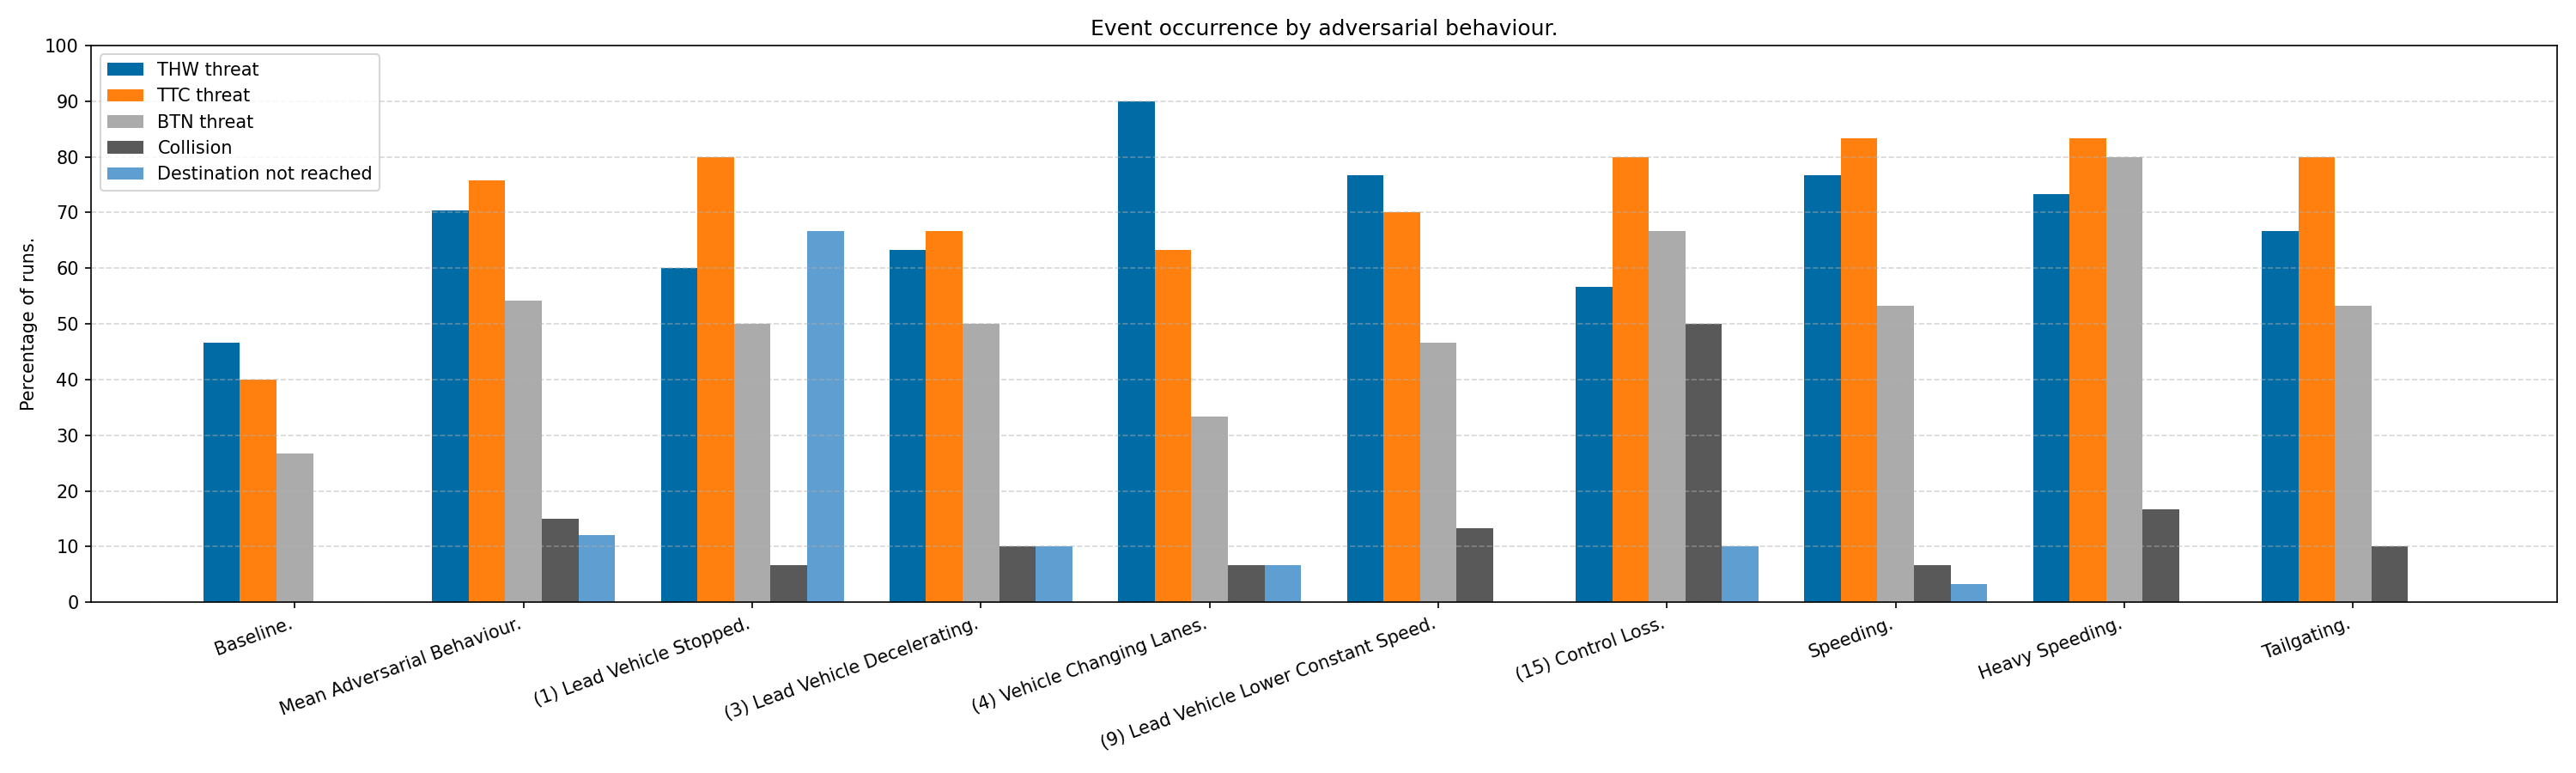
\includegraphics[width=1\linewidth]{imgs/rdb_events.png}
          \caption{Event occurrence by adversarial behaviour, roundabouts.}
          \label{fig:rdb_events}
\end{figure*}

\fi










\endinput
%%
%% End of file `sample-sigconf.tex'.


\section{Related Work}


\iffalse
We first review existing work in scenario-based ADS testing and adversarial scenario generation, identifying the gap that motivates our approach (Sec.~\ref{sec:scenario_based_testing}--\ref{sec:scenario_generation}). We then introduce the simulation platforms and ADS used in our project (Sec.~\ref{sec:platform_ads}), followed by the two external frameworks --- the NHTSA pre-crash scenario typology and the Euro NCAP assisted driving protocol --- that ground our methodology in real-world crash statistics and regulatory kinematic standards (Sec.~\ref{sec:NHTSA}--\ref{sec:euro_ncap}).

\subsection{Scenario-Based Testing of ADS}\label{sec:scenario_based_testing}

Simulation-based testing has become the dominant paradigm for ADS evaluation. Kalra and Paddock~\cite{kalra_driving_2016} demonstrated that proving the statistical safety of an autonomous vehicle would require over $10^9$ miles of on-road driving --- an impractical requirement that has driven the community towards virtual, scenario-based evaluation. High-fidelity simulators such as CARLA~\cite{dosovitskiy_carla_2017} and LGSVL~\cite{rong_lgsvl_2020} provide controllable virtual environments with realistic sensor models, physics, and rendering, but their effectiveness depends critically on the quality, diversity, and realism of the test scenarios they execute.

Several naturalistic driving datasets have been developed to populate simulation testing pipelines. The inD dataset~\cite{bock_ind_2020} provides drone-recorded vehicle and pedestrian trajectories at German intersections, while highD~\cite{krajewski_highd_2018} captures highway traffic and rounD~\cite{krajewski_round_2020} records roundabout interactions. The Waymo Open Dataset~\cite{sun_scalability_2020} and nuScenes~\cite{caesar_nuscenes_2020} supply large-scale multi-sensor data from urban driving. The CARLA Leaderboard~\cite{noauthor_carla_nodate} defines ten traffic scenarios derived from the NHTSA pre-crash typology, providing a standardized benchmark for end-to-end ADS evaluation. The SCTrans dataset~\cite{dai_sctrans_2024}, which we use as the basis for our seed scenario identification, constructs over 1,900 simulation scenarios by transforming naturalistic traffic recordings into OpenSCENARIO files compatible with CARLA and LGSVL. SCTrans demonstrated that its scenarios can boost the collision-finding capability of existing ADS fuzzers by approximately seven times. However, a fundamental limitation shared by all these datasets is that they model \textit{well-behaved} traffic participants whose actions conform to expected driving norms, leaving adversarial edge cases underrepresented.

Scenario generation methods span three broad categories~\cite{wang_survey_2024, riedmaier_survey_2020, tang_survey_2023}. \textit{Rule-based methods} rely on expert knowledge, traffic regulations, and ontologies to derive test scenarios. Deng et al.~\cite{deng_target_2025} (TARGET) use LLM-guided knowledge extraction from traffic rules to generate test scenarios and evaluate seven ADS across CARLA, LGSVL, and MetaDrive. Birkemeyer et al.~\cite{birkemeyer_feature-interaction_2022} apply combinatorial testing with feature-interaction sampling for ADAS testing. While systematic, these approaches are constrained to scenarios that conform to predefined rules and expert expectations.

\textbf{Data-driven approaches} extract or synthesize scenarios from naturalistic data. TrafficGen~\cite{feng_trafficgen_2023} learns to generate diverse and realistic traffic scenarios, while TrafficComposer~\cite{tu_multi-modal_2025} combines natural language descriptions with traffic scene images for multi-modal scenario construction. Jia et al.~\cite{ji_effuzz_2023} use conditional generative adversarial imitation learning to produce different types of traffic scenarios. These methods are effective at reproducing realistic traffic distributions but inherit the bias of their training data --- since safety-critical events are extremely rare in naturalistic driving, data-driven methods tend to generate predominantly safe scenarios.

\textbf{Search-based methods} formulate generation as an optimization problem. AV-FUZZER~\cite{li_av-fuzzer_2020} uses genetic algorithms to search for NPC manoeuvres that lead to ADS safety violations, employing a fitness function based on safety potential. DriveFuzz~\cite{kim_drivefuzz_2022} extends fuzzing to the full ADS stack by mutating maps, actors, weather, and road conditions, discovering 30 bugs in Autoware and CARLA Behavior Agent. TM-fuzzer~\cite{lin_tm-fuzzer_2024} improves upon DriveFuzz by strategically managing NPC vehicle placement through a traffic management engine, achieving superior violation discovery. OSG~\cite{yan_-demand_2025} generates scenarios across varying risk levels using a Risk Intensity Regulator and speciation-based particle swarm optimization, providing a comprehensive ADS scoring system. EF-Fuzz~\cite{ji_effuzz_2023} introduces risk-guided seed selection, achieving a 37.9\% efficiency increase over DriveFuzz. ISS-Scenarios~\cite{li_iss-scenario_2024} provides a parameterized scenario library for batch testing in CARLA with both random sampling and genetic-algorithm-based search.

While effective at finding collision-inducing \textbf{configurations}, these search-based approaches treat external vehicle behaviour as a secondary search dimension --- mutating positions, speeds, or spawn locations rather than systematically modelling specific types of adversarial driving behaviour. The generated scenarios may expose bugs but often produce unrealistic NPC actions that do not correspond to plausible real-world driver behaviour.

\subsection{Adversarial and Safety-Critical Scenario Generation}\label{sec:scenario_generation}

A growing body of work specifically targets safety-critical scenarios through adversarial methods, which can be organized into three categories.
All three categories have the follwing key limitations: adversarial scenarios are very short in duration restricted to 5 seconds or less, narrow in scope focussingg on simple vehicle interactions in a very simple setting like a junction or single lane and finally lacking connection with realistic vehicle interactions that lead to collisions and other forms of undesirable behaviour. 

\textbf{Reinforcement learning approaches} train adversarial agents to challenge the ego vehicle. Learning-to-Collide~\cite{ding_learning_2020} represents traffic scenarios as autoregressive building blocks and trains a generative agent via policy gradient methods to search for risky scenario parameters. Feng et al.~\cite{feng_dense_2023} develop a dense deep reinforcement learning (D2RL) approach that edits Markov decision processes to densify safety-critical information, enabling naturalistic and adversarial environment generation. The CRASH framework~\cite{kulkarni_crash_2024} uses adversarial deep RL to control NPC agents, inducing collisions with the ego vehicle and iteratively refining the motion planner through safety hardening. AuthSim~\cite{yang_authsim_2025} proposes a three-layer relative safety region model combined with RL to ensure that generated scenarios are \textit{authentic} --- the ego vehicle bears primary collision responsibility rather than NPCs engaging in physically implausible attacks.

While RL-based approaches can discover effective adversarial strategies, they face several limitations: (1) they typically operate in narrow scenario classes (e.g., highway merging or single-lane following) rather than covering a comprehensive pre-crash typology; (2) they require extensive training time and computational resources; (3) the learned adversarial policies may produce behaviours that, while collision-inducing, do not correspond to recognizable real-world driving errors; and (4) they generally do not provide the kinematic interpretability needed to classify discovered vulnerabilities against established crash typologies.

\textbf{Trajectory perturbation approaches} directly modify actor trajectories. AdvSim~\cite{wang_advsim_2023} perturbs trajectories in a physically plausible manner and updates LiDAR sensor data to match the perturbed world, generating safety-critical scenarios for the full LiDAR-based autonomy stack. STRIVE~\cite{rempe_generating_2022} optimizes adversarial trajectories in the latent space of a VAE model to generate accident-prone driving scenarios. DiffScene~\cite{xu_diffscene_2025} applies diffusion models for safety-critical scenario generation, while CausalAF~\cite{ding_causalaf_2023} uses causal autoregressive flows. Game-theoretic methods~\cite{lin_scenario-based_2025} model adversarial vehicle interactions using kinematic constraints and reachable-set analysis. These methods can produce diverse scenarios but are typically limited to simplified driving environments, pairwise vehicle interactions, or lack systematic coverage of the full spectrum of pre-crash typologies.

\textbf{LLM and foundation model approaches} represent the most recent trend. ChatScene~\cite{zhang_chatscene_2024} uses knowledge-enabled LLMs for safety-critical scenario generation, outperforming prior methods across multiple ego vehicles and base scenarios. ScenGE~\cite{liu_adversarial_2025} combines LLM-based meta-scenario generation with retrieval-augmented grounding in traffic regulations and pre-crash scenario knowledge, using a structured knowledge base to ensure both plausibility and criticality. The retrieval-augmented framework by Nie et al.~\cite{mei_seeking_2025} employs an LLM-based behaviour analyser to infer the most dangerous intent of background vehicles and synthesize adversarial trajectories. SafeBench~\cite{xu_safebench_2022} provides a benchmarking platform integrating multiple generation algorithms (Learning-to-Collide, AdvSim, Adversarial Trajectory Optimization) with multiple ADS, though its predefined scenario types do not systematically cover the full NHTSA pre-crash typology.



\fi

A growing body of work targets safety-critical scenarios through adversarial methods, broadly spanning three categories. Across all categories, however, existing approaches share key limitations: scenarios are short in duration (typically $\leq5$ seconds), narrow in scope (e.g., simple junctions or single-lane interactions), and weakly grounded in realistic, complex vehicle behaviours that lead to real-world collisions.

Reinforcement learning approaches train adversarial agents to challenge the ego vehicle (e.g., Learning-to-Collide~\cite{ding_learning_2020}, D2RL~\cite{feng_dense_2023}, CRASH~\cite{kulkarni_crash_2024}, AuthSim~\cite{yang_authsim_2025}). While effective at inducing failures, they are typically confined to narrow scenario classes, require significant training cost, and often produce behaviours that lack realism or kinematic interpretability, limiting alignment with established crash typologies.

Trajectory perturbation approaches directly modify actor trajectories (e.g., AdvSim~\cite{wang_advsim_2023}, STRIVE~\cite{rempe_generating_2022}, DiffScene~\cite{xu_diffscene_2025}, CausalAF~\cite{ding_causalaf_2023}, game-theoretic methods~\cite{lin_scenario-based_2025}). Although they enable diverse scenario generation, they are generally restricted to simplified environments or pairwise interactions and do not provide systematic coverage of pre-crash scenarios.

LLM and foundation model approaches (e.g., ChatScene~\cite{zhang_chatscene_2024}, ScenGE~\cite{liu_adversarial_2025}, retrieval-augmented methods~\cite{mei_seeking_2025} , SafeBench~\cite{xu_safebench_2022}) improve diversity and plausibility through knowledge grounding. However, they still inherit limitations in scenario duration, interaction complexity, and systematic coverage of real-world pre-crash typologies.
\section{Conclusion}
This paper presents an adversarial scenario generation approach that manipulates the trajectories of external vehicles, grounded in pre-crash interaction typologies documented by NHTSA. We further introduce the first adversarial scenario generation pipeline specifically targeting roundabout environments.
Evaluation across 300 adversarial scenarios for both regular and roundabout settings demonstrates a substantial increase in triggered threats, collisions, and failure-to-reach-destination events for Apollo and TM, compared to baseline scenarios assuming well-behaved external vehicles.
These results expose concrete and reproducible failure modes in current autonomous driving systems, underscoring critical challenges for safety certification and raising important considerations for their readiness for public deployment.
\section{Dataset Availability}
The source code for the approach and the generated adversarial scenarios are available at
\url{https://anonymous.4open.science/r/AVESGen-22D6/}

\noindent To preserve public disclosure of code and artifacts during review phase and protecting ourselves from reuse of our code before our work is published, we provide a private anonymous link rather than a public DOI-backed repository. Upon acceptance, the artifact will be made publicly available with a DOI.

% \section{Dataset Availability}
% The source code for the approach and the generated adversarial scenarios are available at \\
% \hyperlink{github link}{https://anonymous.4open.science/r/AVESGen-22D6/}
\newpage
\bibliographystyle{plainnat}
\bibliography{references}
\end{document}
\endinput
%%
%% End of file `sample-sigconf.tex'.
